%% ============================================================
%% body.tex — 팀 구성 + 1~4일차 진행 (사진 27장 전수 + 부록 발췌)
%% ============================================================

\section{팀 구성 및 주요 업무}
교수진과 제품개발학기 참여 학생의 역할 분담은 다음과 같다. 서비스 애플리케이션,
시뮬레이션, 펌웨어, UI/UX, 실물 교구 디자인을 나누어 진행한다.

\subsection*{교수진}
\begin{center}
\renewcommand{\arraystretch}{1.35}
\begin{tabularx}{\linewidth}{@{}>{\sffamily\bfseries}l L{0.72\linewidth}@{}}
\toprule
\sffamily 강영민 & 서비스 애플리케이션 개발 \\
\sffamily 서미라 & 제품 디자인 지도 (실물 교구 및 온라인 서비스) \\
\sffamily 신\,\,원 & 제품개발학기 총괄 진행 및 제품 수준의 서비스 관리 \\
\bottomrule
\end{tabularx}
\end{center}

\subsection*{학생}
\begin{center}
\renewcommand{\arraystretch}{1.35}
\begin{tabularx}{\linewidth}{@{}>{\sffamily\bfseries}l L{0.72\linewidth}@{}}
\toprule
\sffamily 김지훈 & 시뮬레이션 모듈 고도화 및 디지털 트윈 시스템 구현 \\
\sffamily 이민혁 & 시뮬레이션 모듈 고도화 및 디지털 트윈 시스템 구현 \\
\sffamily 이주현 & 펌웨어 개발 및 블록코딩 서비스 연계 \\
\sffamily 이성빈 & 제품 서비스 UI/UX 고도화 \\
\sffamily 이재훈 & 실물 교구 디자인 기획 및 시작품 제작 \\
\bottomrule
\end{tabularx}
\end{center}

% ============================================================
\section{1일차 — 컴퓨터실 개발 착수}
\textit{2026.06.23 (월) · 10:00\,--\,17:00 KST}

\begin{summarybox}
컴퓨터실에서 개발에 착수했다. 로버 하드웨어(섀시$\cdot$모터 컨트롤러 보드)를
조립하고, 발사대$\cdot$로켓$\cdot$LED 모형을 제작했으며, 블록 코딩과 펌웨어 작업을
병행했다. 동시에 저장소 전체를 코드 수준에서 분석한 종합 보고서를 작성했다.
\end{summarybox}

\subsection{주요 업무 — 코드 분석 종합 보고서 작성}
ARES 저장소~\cite{ares-repo} 전체를 코드 수준에서 분석한 \textbf{「ARES 프로젝트
코드 분석 종합 보고서」(전 14장)}를 작성했다. 웹$\cdot$펌웨어$\cdot$AI 세 런타임
도메인이 \emph{개행 구분 텍스트 명령}이라는 단일 계약으로 느슨하게 결합되는
구조를 중심으로, 하드웨어부터 향후 연구 방향까지 망라했다. 핵심 내용은 본문
「산출물」에 요약하고, 전문은 부록~\ref{app:code}에 수록한다.

\smallskip
\noindent\chip{개요·구성요소}~\chip{하드웨어·핀 배치}~\chip{피코 펌웨어}~%
\chip{웹 서비스 계층}~\chip{Web Bluetooth}~\chip{블록 코딩}~\chip{WebGL 3D 시뮬레이션}

\begin{itemize}
  \item \textbf{대상 시스템} — 초등학생용 블록 코딩 화성 탐사 로버 ‘알비’:
  Blockly 웹앱~\cite{blockly} + 라즈베리파이 피코(MicroPython) 펌웨어 + AI 보조 모듈.
  \item \textbf{핵심 발견} — 웹과 펌웨어는 코드를 공유하지 않고 \emph{텍스트 명령
  프로토콜}만으로 통신해 독립 개발$\cdot$교체가 쉬운 반면, 프로토콜 변경 시 양측
  동시 반영 의존이 생긴다.
  \item \textbf{범위} — 블록 1개가 ‘블록 → 명령 문자열 → BLE → 펌웨어 핸들러 →
  하드웨어’로 도달하는 전 경로를 코드로 추적.
\end{itemize}

%% ---- 부록 발췌 1: 데이터 흐름 ----
\begin{diagram}{데이터 흐름 — 블록에서 하드웨어까지 (부록~\ref{app:code} 발췌)}{fig:dataflow}
  \node[dom] (web) {웹 UI\\\footnotesize Blockly};
  \node[box, right=12mm of web] (ble) {Web Bluetooth\\\footnotesize 20B 청크};
  \node[dom, right=12mm of ble] (pico) {피코 펌웨어\\\footnotesize CommandProcessor};
  \node[hw, right=12mm of pico] (hw) {하드웨어\\\footnotesize 모듈};
  \draw[flow] (web) -- node[lbl, above]{명령 문자열} (ble);
  \draw[flow] (ble) -- node[lbl, above]{UART 9600} (pico);
  \draw[flow] (pico) -- (hw);
  \draw[back] (pico.south) to[bend left=28] node[lbl, below]{응답(DIST:/MAG: 등)} (ble.south);
\end{diagram}

\begin{infobox}[title=부록 A 발췌 --- 세 런타임 도메인]
\small
\textbf{웹 UI}(\code{Web/}) Blockly 블록 코딩 + Web Bluetooth 통신~\cite{webbluetooth}\,/\;
\textbf{피코 펌웨어}(\code{Pico/}) MicroPython, UART/BLE 수신 → \code{CommandProcessor}
디스패치~\cite{rp2040}\,/\; \textbf{AI 보조}(\code{AI/}) EXAONE 기반 로컬 LLM
질의응답~\cite{exaone35}. 세 도메인은 코드를 공유하지 않고 텍스트 명령만으로 결합되며,
\code{API\_DOCUMENTATION.md}가 사실상의 계약 문서다.
\end{infobox}

%% ---- 사진: 1일차 5장 ----
\begin{figure}[H]\centering
  \begin{subfigure}{0.32\linewidth}\centering
    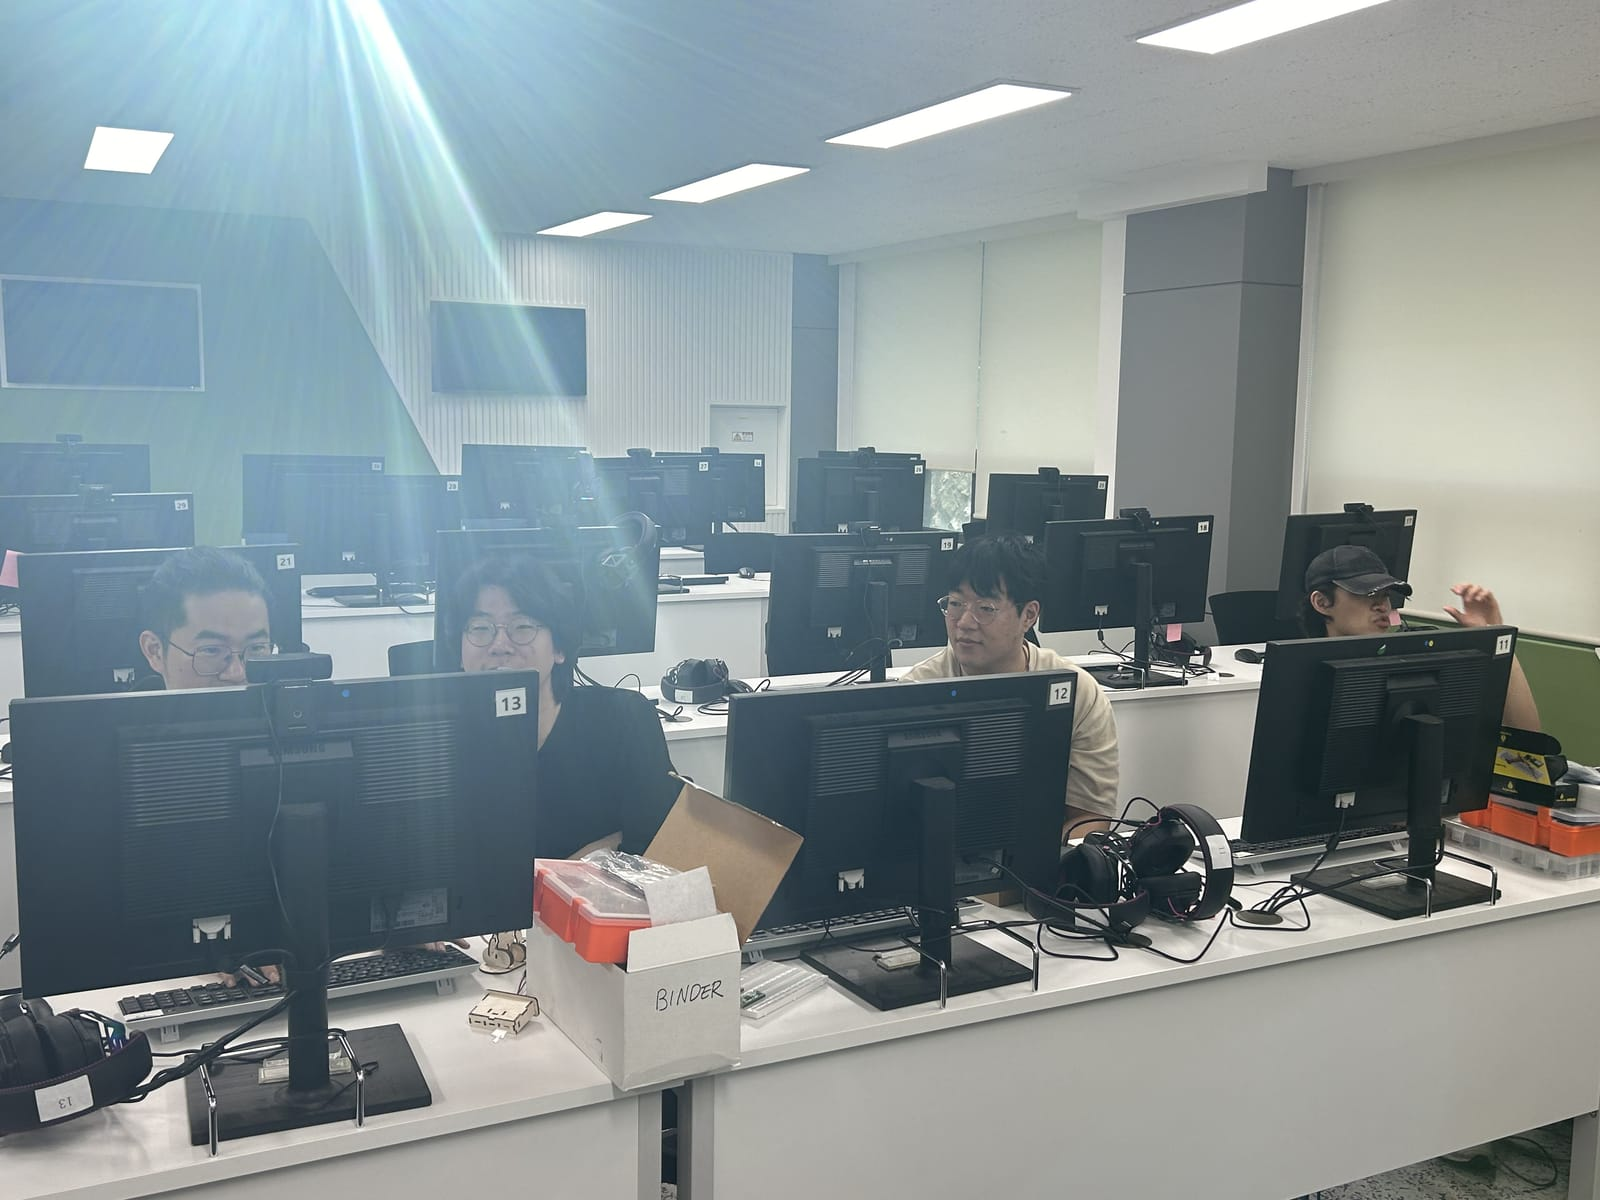
\includegraphics[width=\linewidth, height=4.2cm, keepaspectratio]{../img/1일차_IMG_2948.jpg}
    \caption{개발 착수 (10:32)}
  \end{subfigure}\hfill
  \begin{subfigure}{0.32\linewidth}\centering
    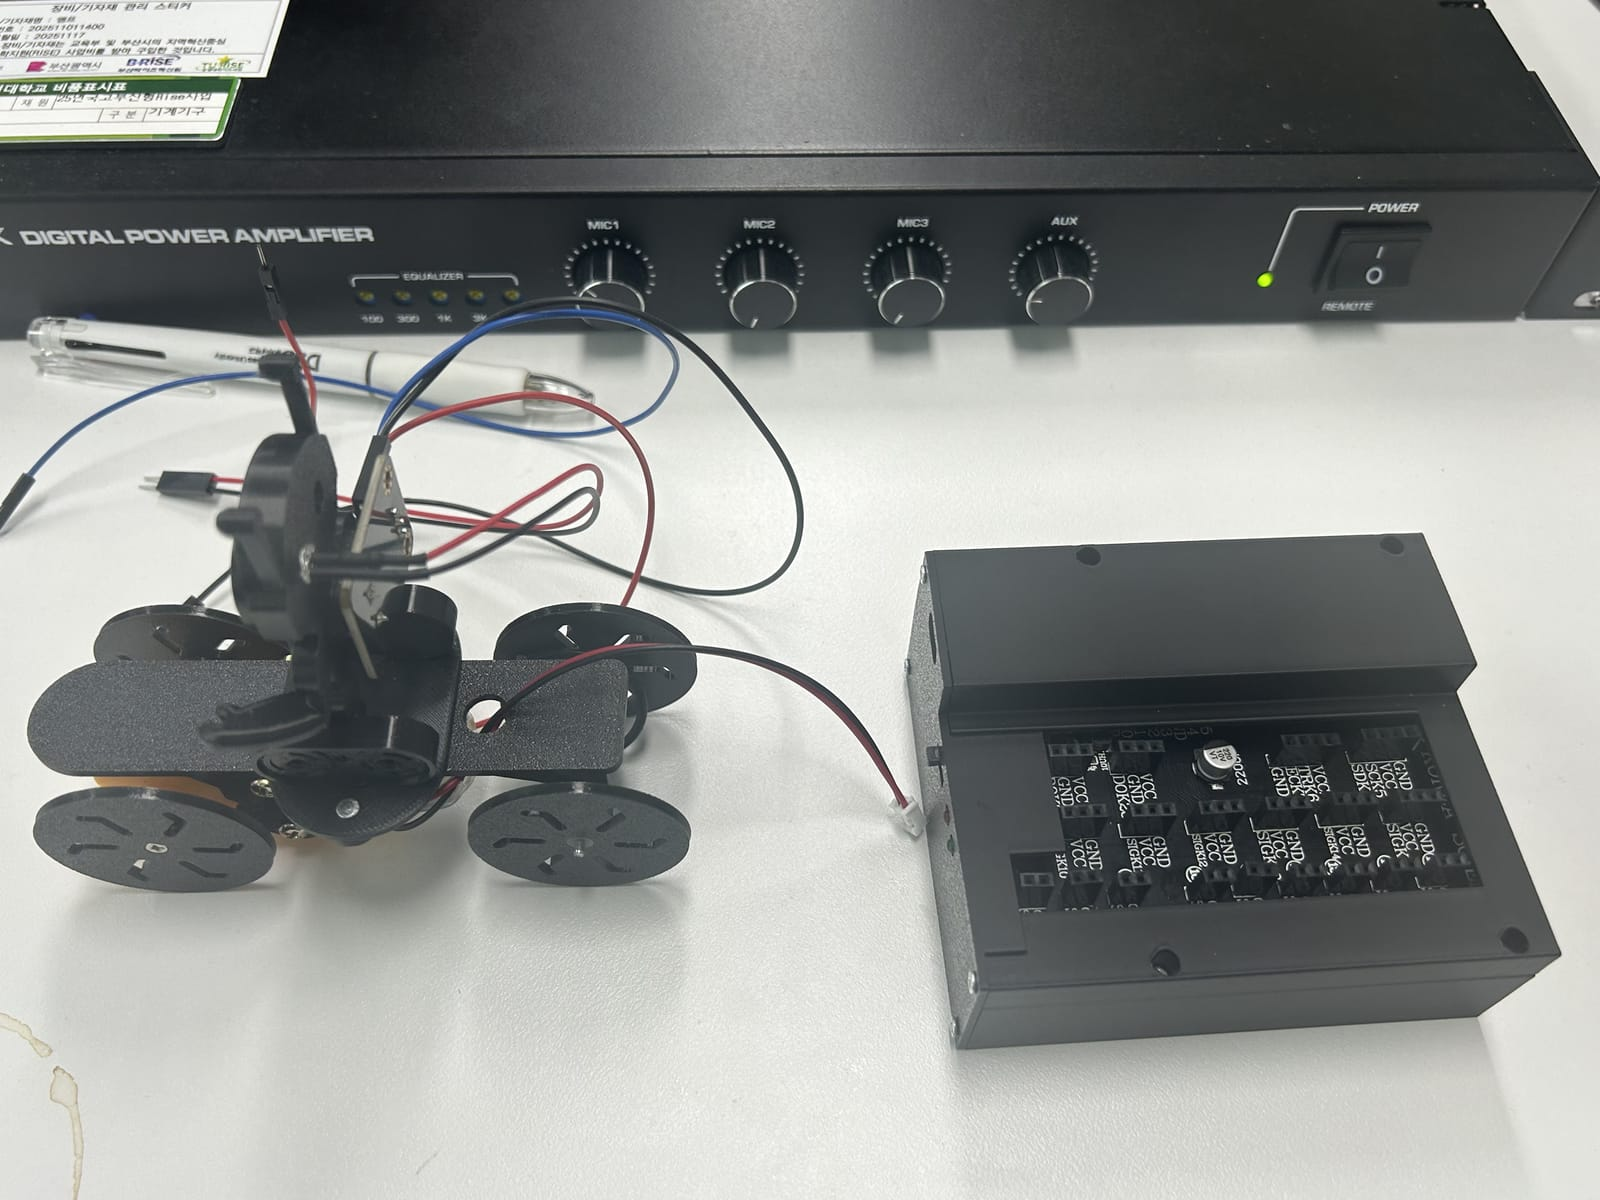
\includegraphics[width=\linewidth, height=4.2cm, keepaspectratio]{../img/1일차_IMG_2949.jpg}
    \caption{4륜 섀시$\cdot$컨트롤러 보드 (11:09)}
  \end{subfigure}\hfill
  \begin{subfigure}{0.32\linewidth}\centering
    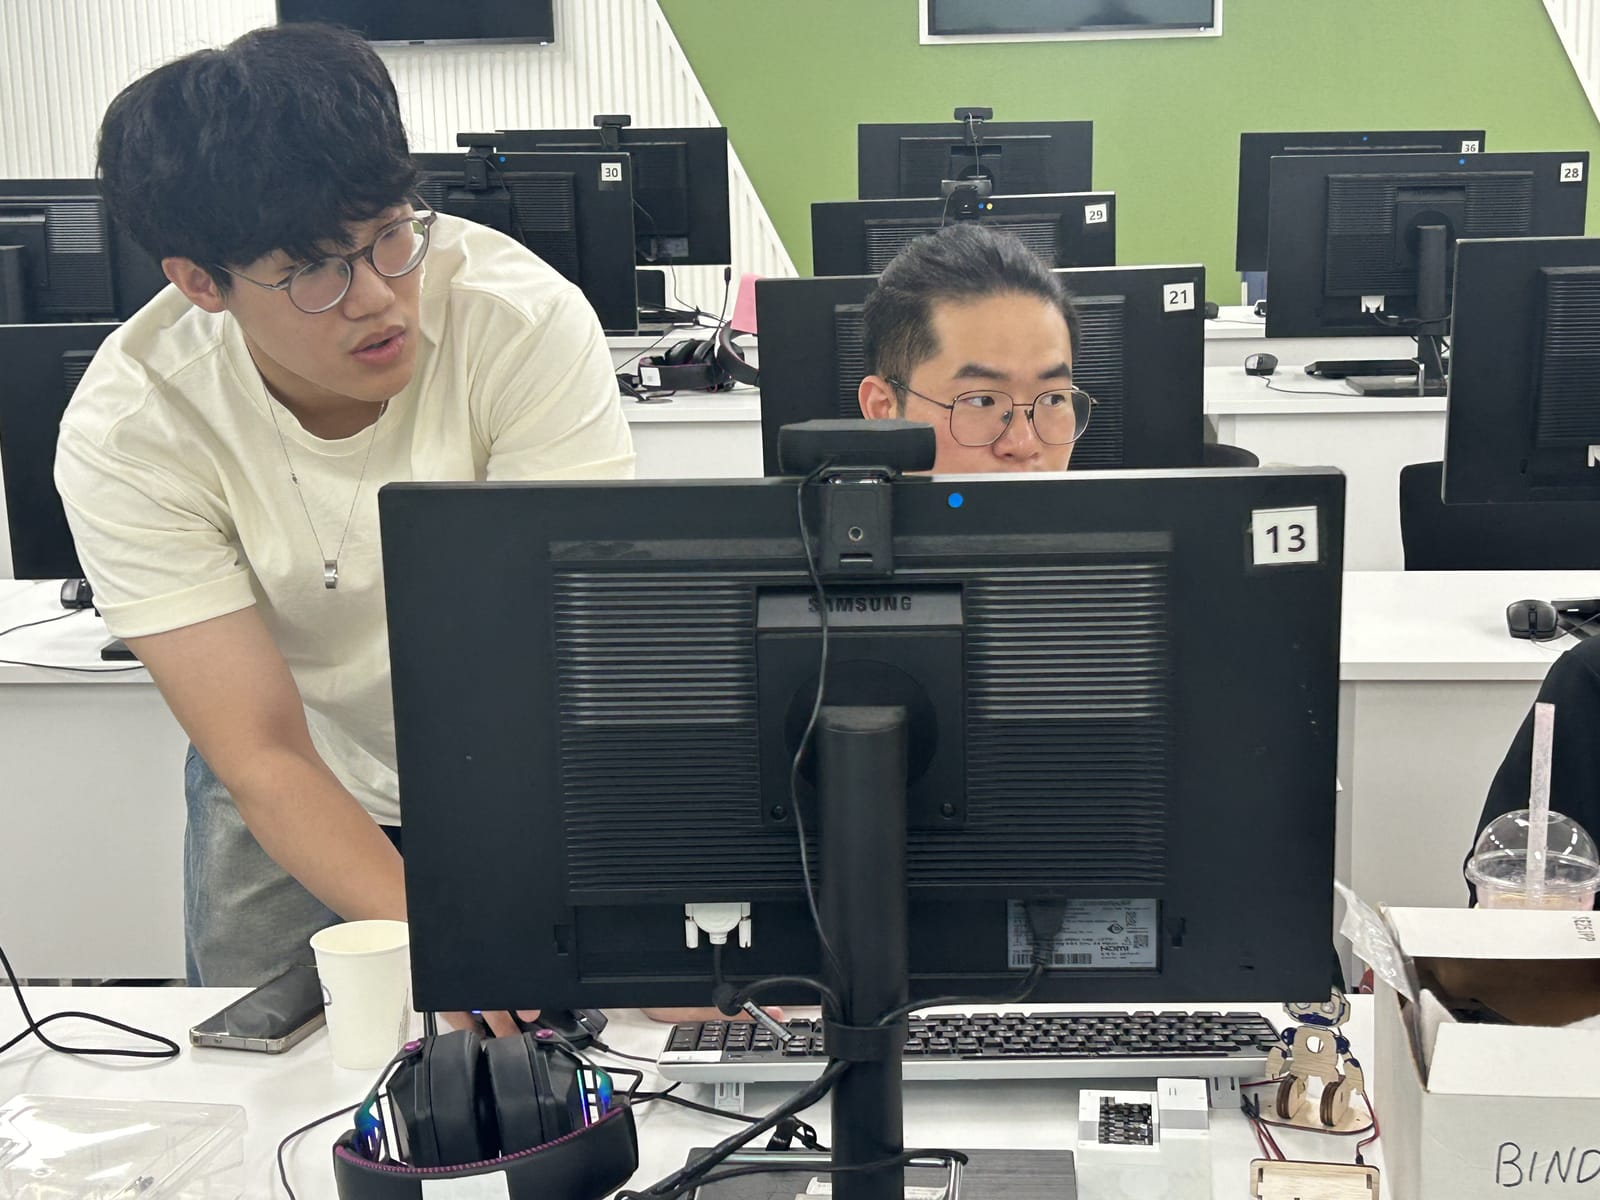
\includegraphics[width=\linewidth, height=4.2cm, keepaspectratio]{../img/1일차_IMG_2951.jpg}
    \caption{페어 작업 (13:30)}
  \end{subfigure}

  \medskip
  \begin{subfigure}{0.32\linewidth}\centering
    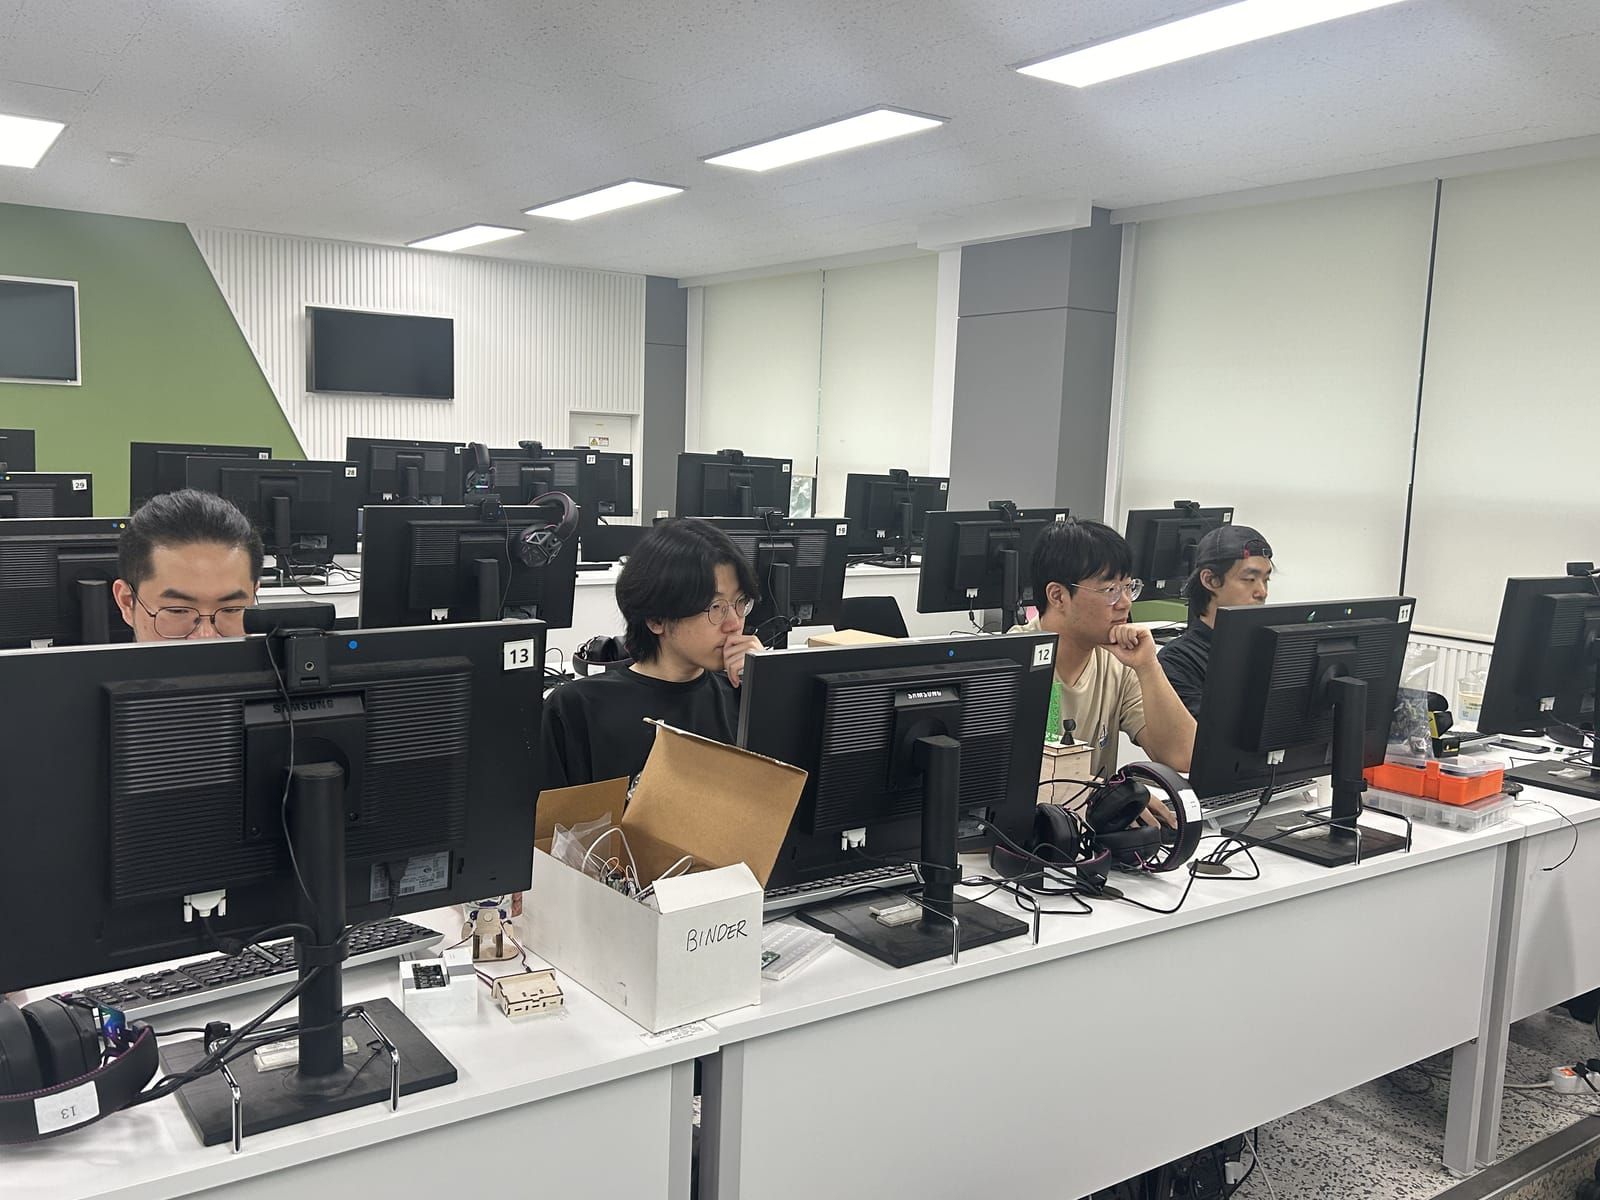
\includegraphics[width=\linewidth, height=4.2cm, keepaspectratio]{../img/1일차_IMG_2952.jpg}
    \caption{컴퓨터실 전경 (13:58)}
  \end{subfigure}\hfill
  \begin{subfigure}{0.32\linewidth}\centering
    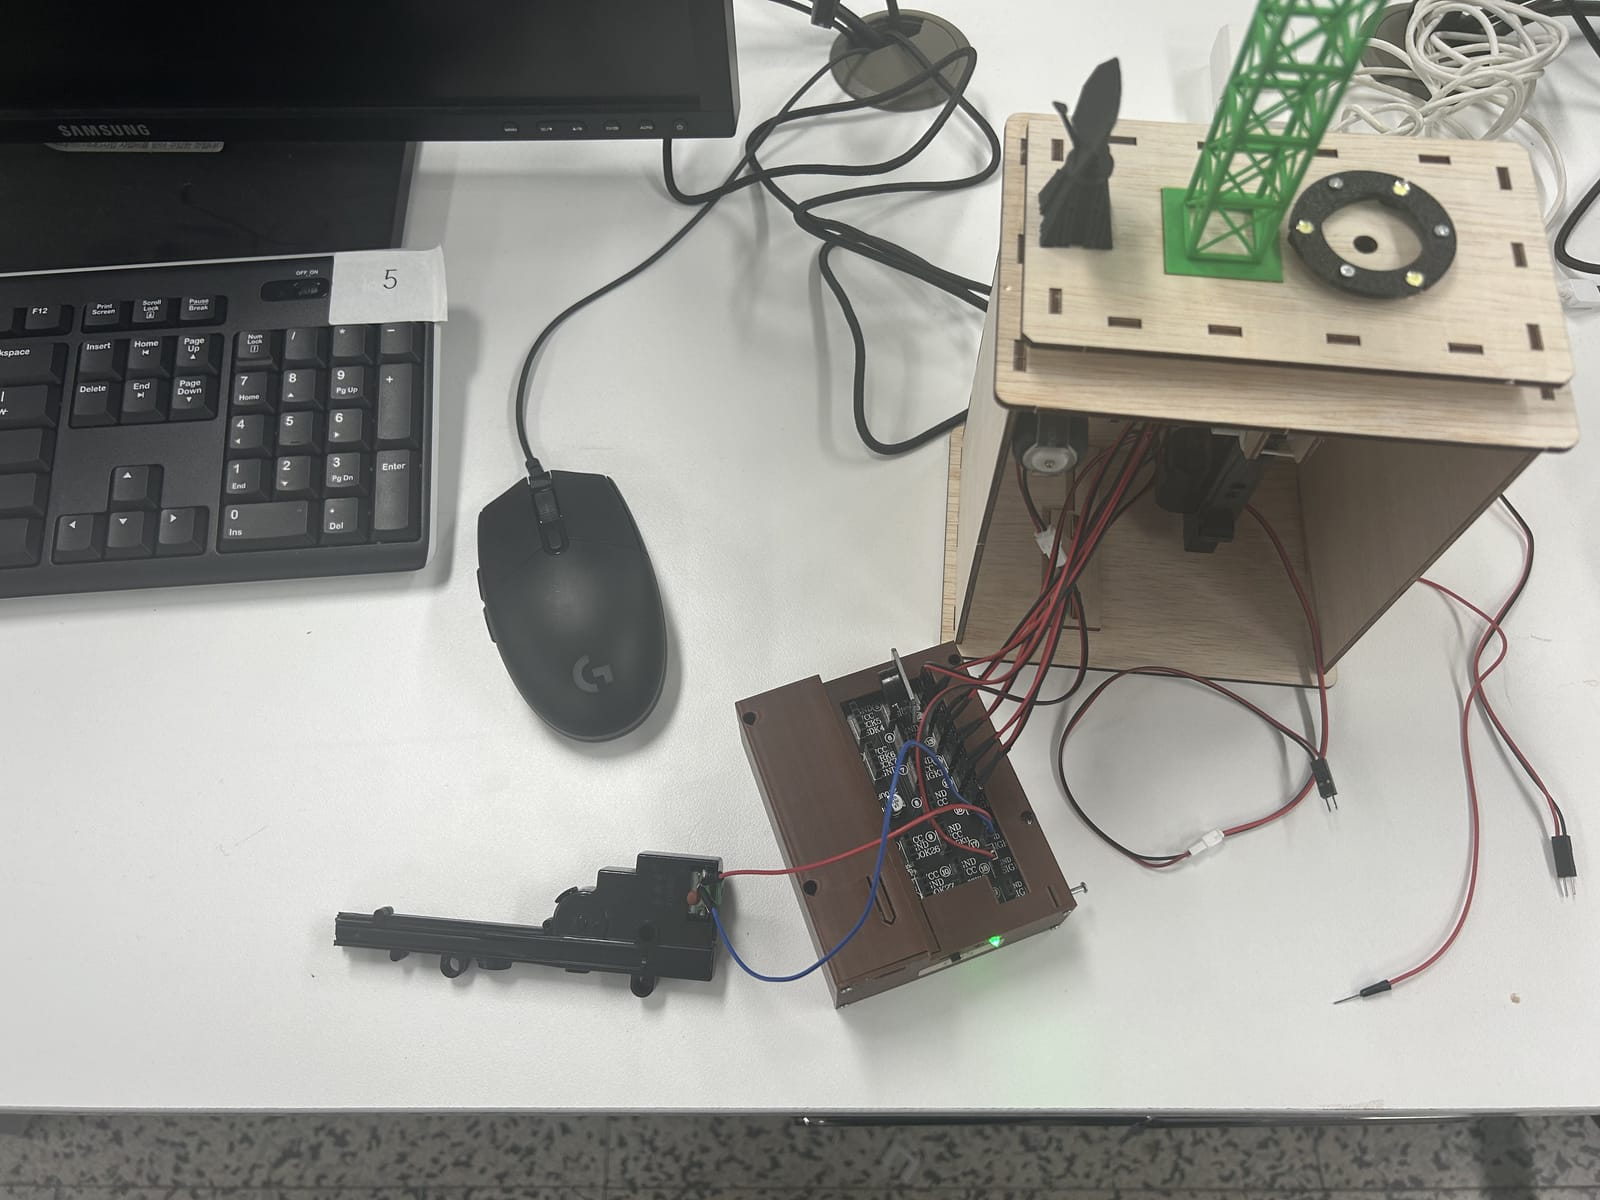
\includegraphics[width=\linewidth, height=4.2cm, keepaspectratio]{../img/1일차_IMG_2955.jpg}
    \caption{발사대 모형 프로토타입 (15:40)}
  \end{subfigure}\hfill
  \begin{subfigure}{0.32\linewidth}\centering\footnotesize
    \vfill\raggedright 4륜 로버 섀시(VCC$\cdot$GND$\cdot$SIG 단자)와 모터 컨트롤러
    보드를 조립하고, 레이저 커팅 목재 발사대에 3D 프린팅 로켓$\cdot$LED 링$\cdot$컨트롤러를
    연결한 하드웨어 프로토타입을 제작했다.\vfill
  \end{subfigure}
  \caption{1일차 — 하드웨어 조립$\cdot$페어 개발과 발사대 모형 제작}
\end{figure}

% ============================================================
\section{2일차 — 제작 협력업체 방문 \& 웹 서비스 시연}
\textit{2026.06.24 (화) · 10:00\,--\,17:00 KST}

\begin{summarybox}
제작 협력업체(D-RISE)의 레이저 커팅 공장을 방문해 키트 부품 생산 공정을
견학하고 재고$\cdot$물류를 협의했다. 이어 회의실에서 ARES 웹 서비스를 시연하고
부품$\cdot$앱의 실제 사용 흐름을 함께 검토했다.
\end{summarybox}

\subsection{주요 업무 — 생산 공정 점검 및 웹 서비스 시연}
키트 양산을 담당하는 제작 협력업체의 레이저 커팅 공장을 방문해 부품 생산
공정을 현장에서 점검하고, 완성된 ARES 블록 코딩 웹 서비스를 관계자에게
시연$\cdot$리뷰했다.

\begin{itemize}
  \item \textbf{생산 공정 견학} — GPL.TECH 레이저 커팅기로 가공되는 목재 키트 부품의
  절단$\cdot$정밀도$\cdot$후처리 공정을 확인.
  \item \textbf{부품$\cdot$재고 점검} — 창고의 키트 부품 재고$\cdot$포장 상태를 보고
  양산$\cdot$물류 일정을 협의.
  \item \textbf{웹 서비스 시연} — 협력업체 관계자에게 ARES 웹 서비스(“블록 코딩으로
  화성을 탐사하다”)를 시연하고 피드백을 수렴, 레이저 커팅 부품과 태블릿 앱의 사용
  흐름을 함께 점검.
\end{itemize}

%% ---- 사진: 2일차 견학 4장 ----
\begin{figure}[H]\centering
  \begin{subfigure}{0.24\linewidth}\centering
    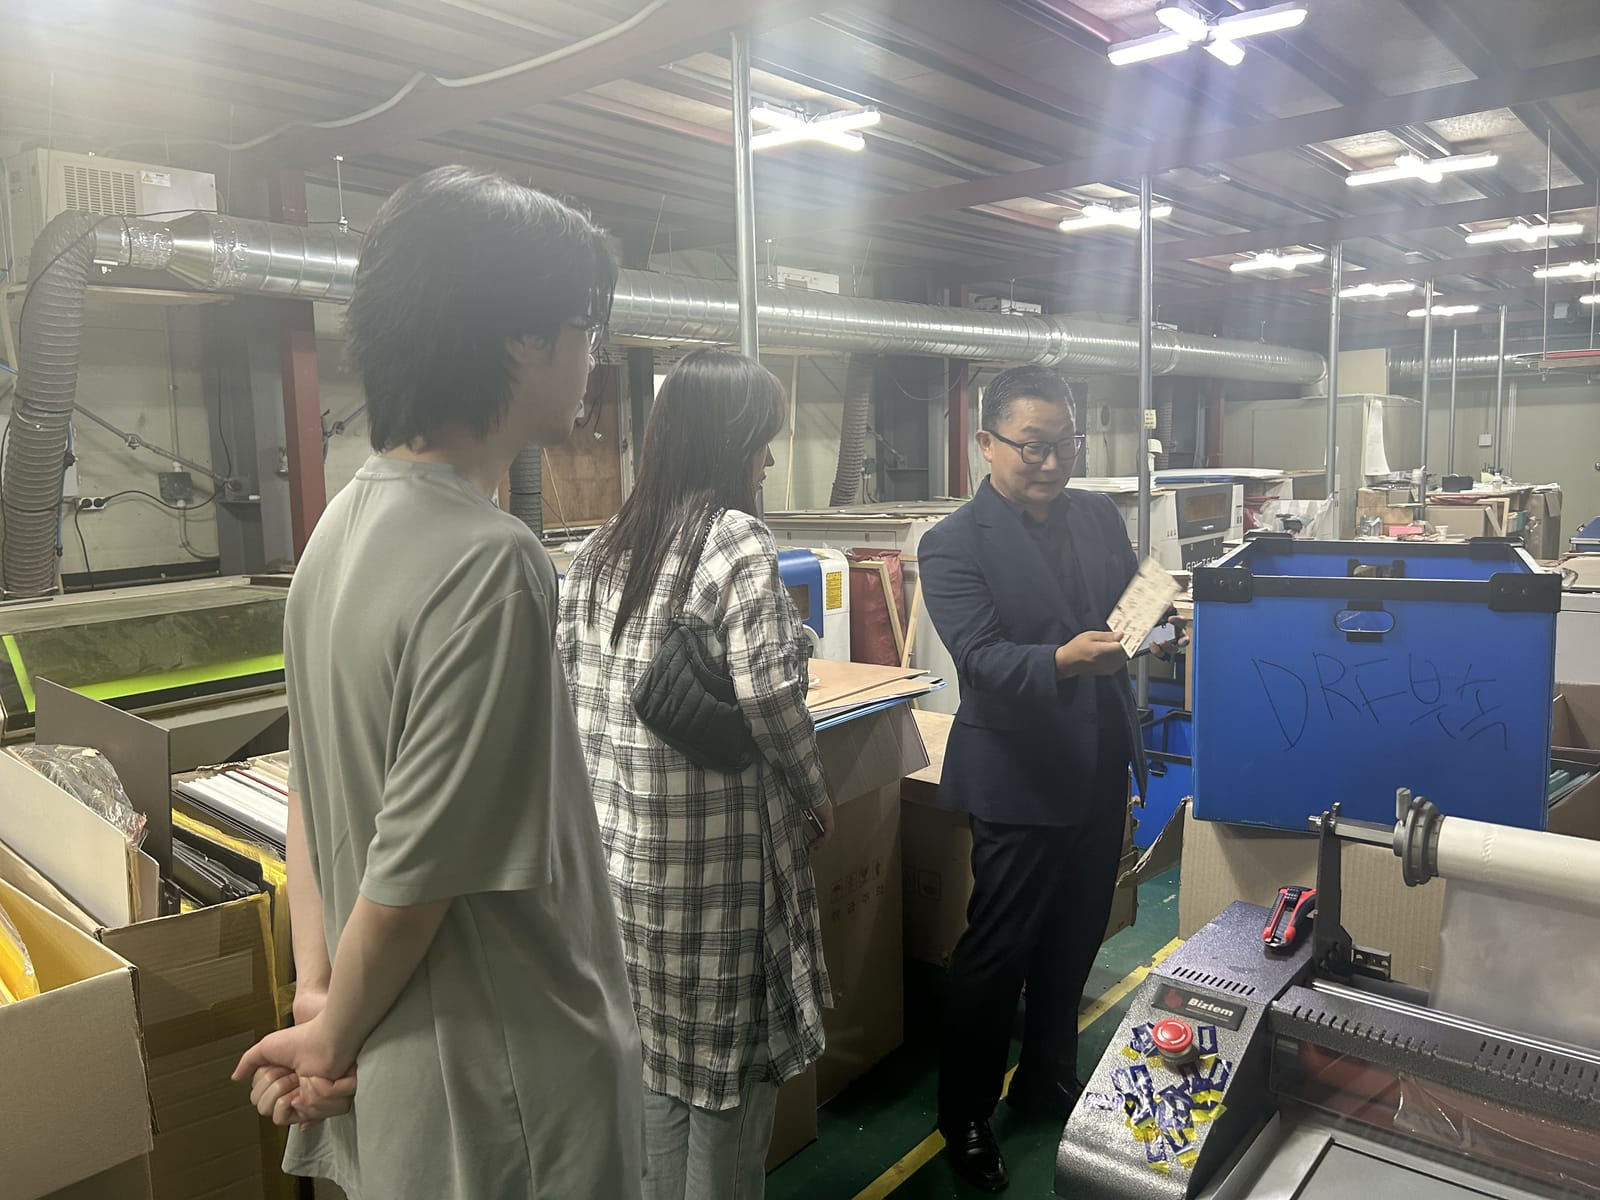
\includegraphics[width=\linewidth, height=3.6cm, keepaspectratio]{../img/2일차_IMG_2961.jpg}
    \caption{부품 설명 (10:44)}
  \end{subfigure}\hfill
  \begin{subfigure}{0.24\linewidth}\centering
    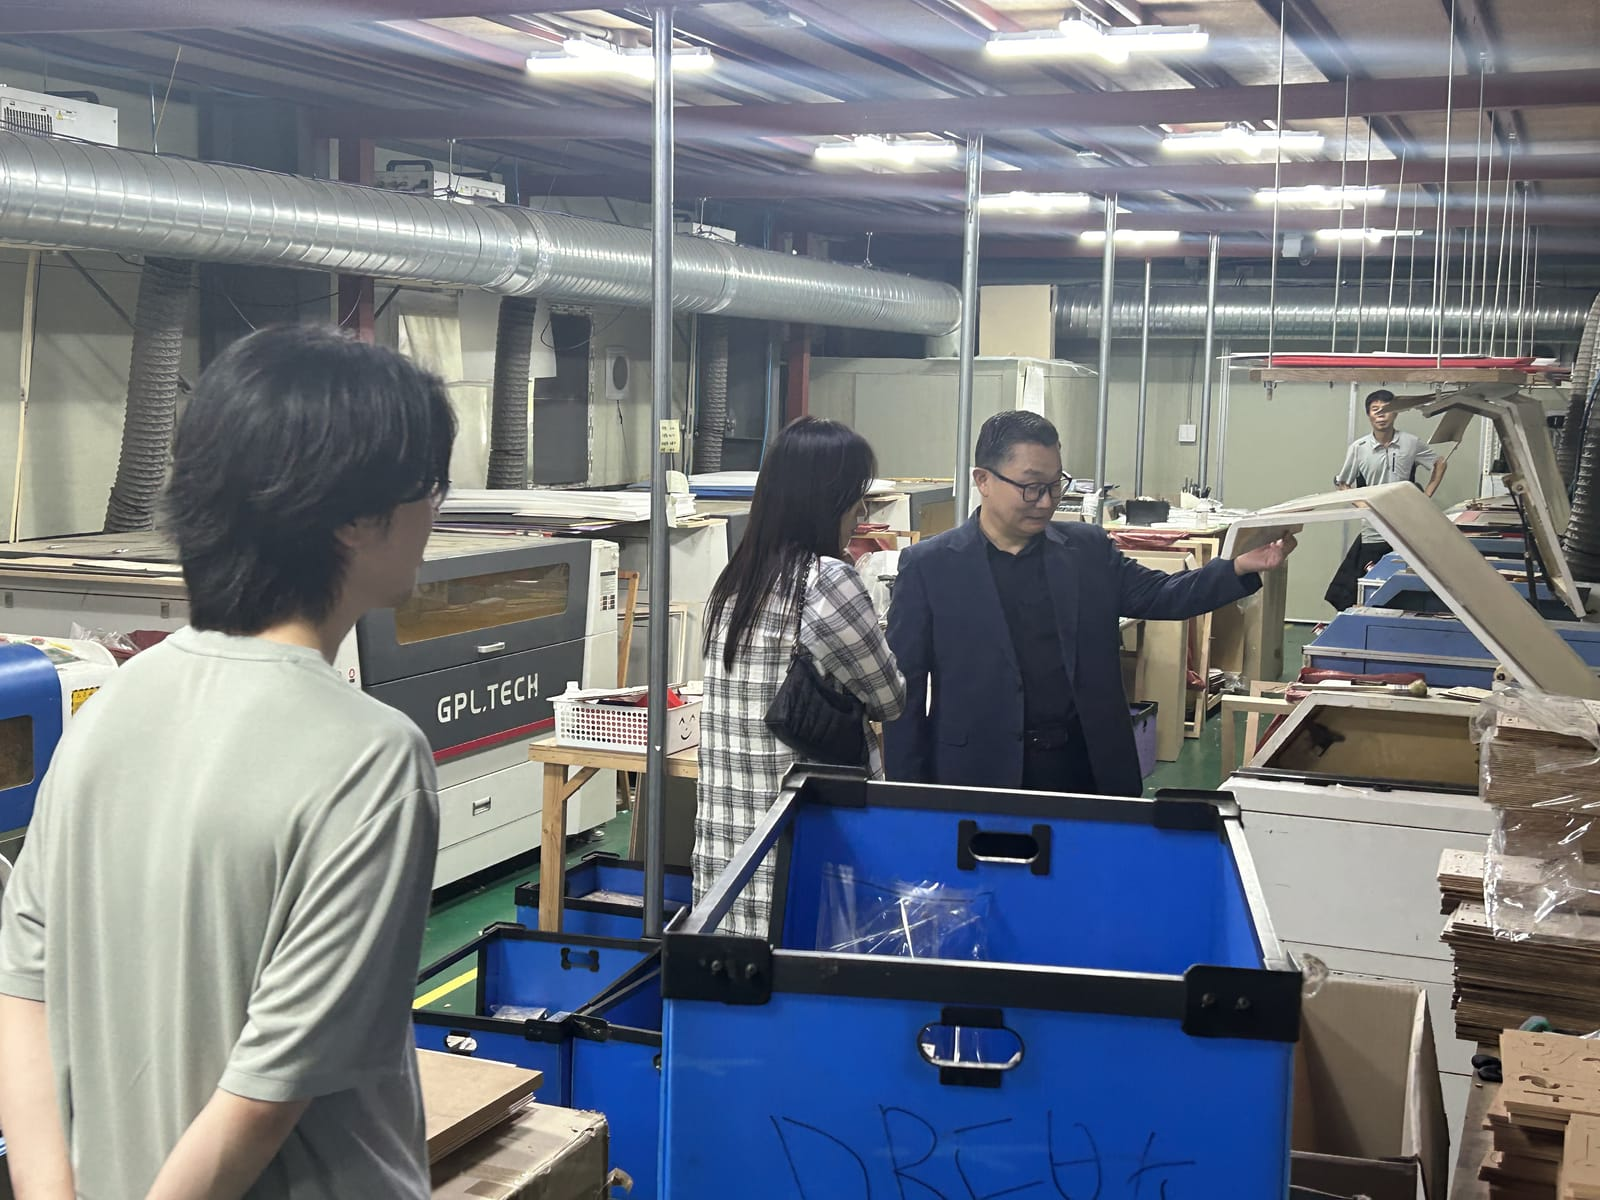
\includegraphics[width=\linewidth, height=3.6cm, keepaspectratio]{../img/2일차_IMG_2962.jpg}
    \caption{커팅기 공정 견학}
  \end{subfigure}\hfill
  \begin{subfigure}{0.24\linewidth}\centering
    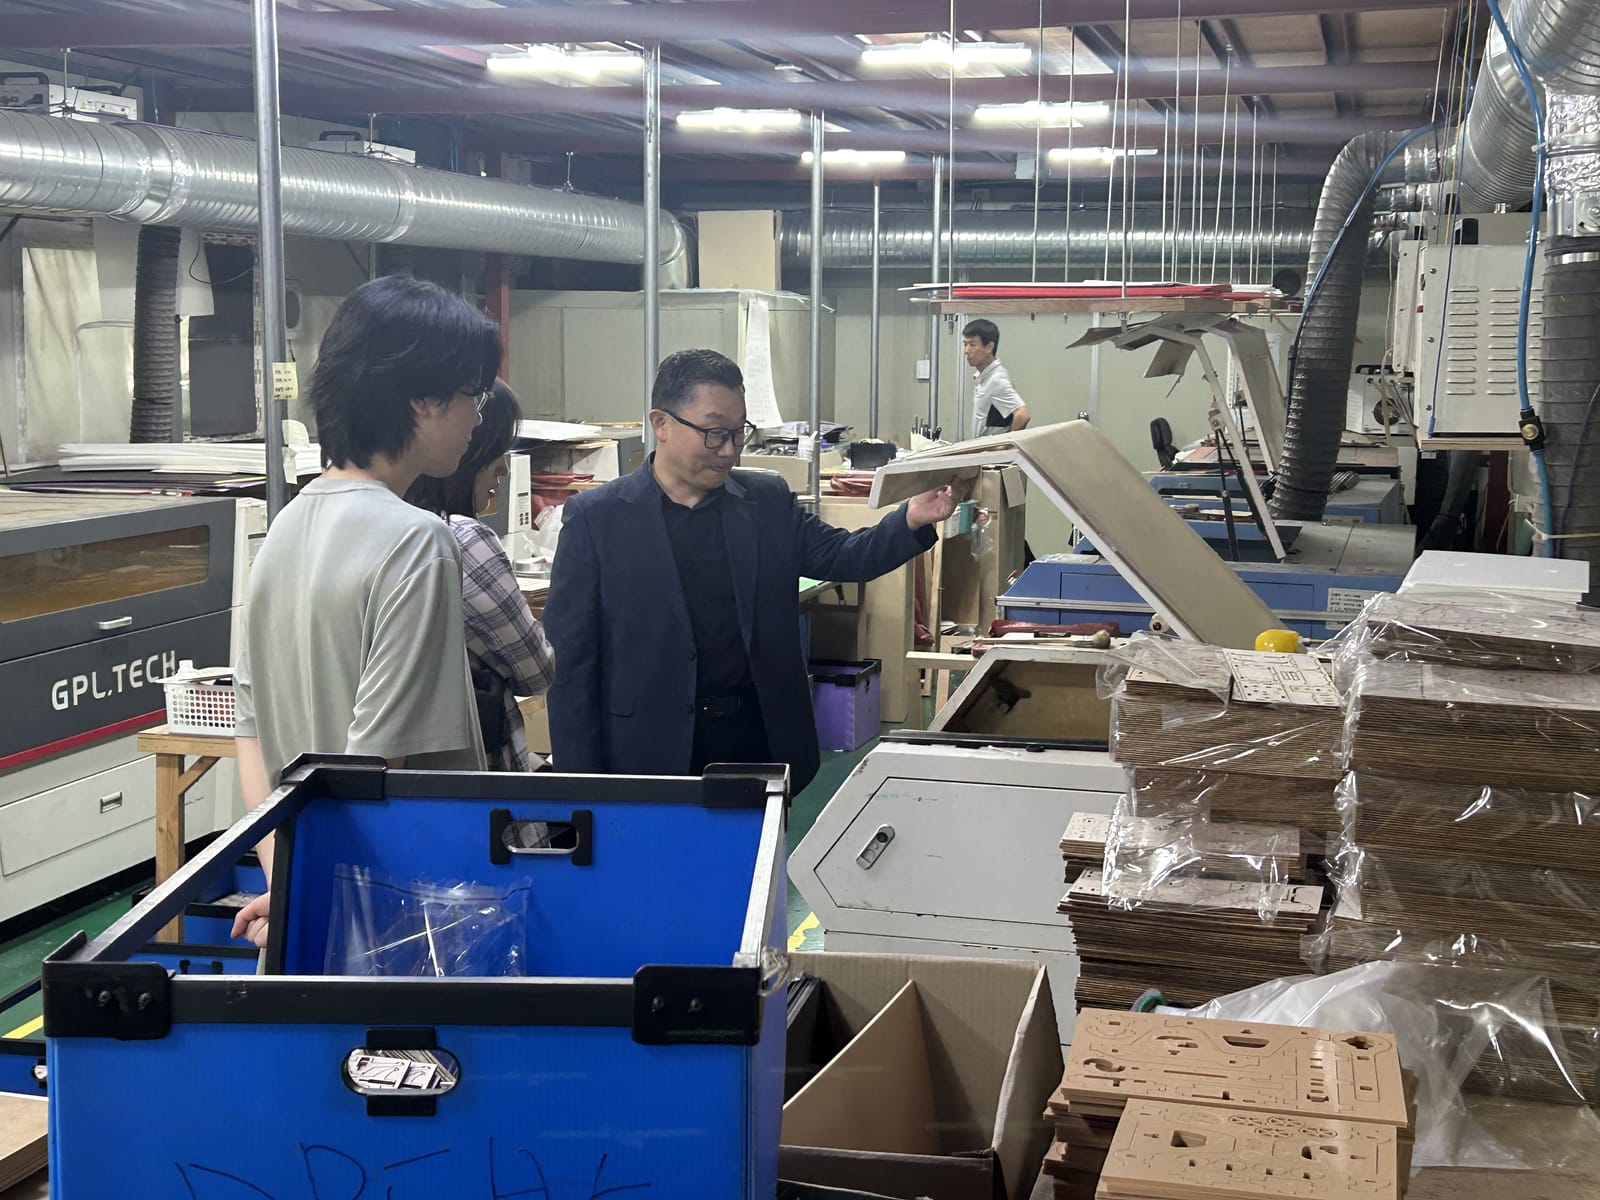
\includegraphics[width=\linewidth, height=3.6cm, keepaspectratio]{../img/2일차_IMG_2963.jpg}
    \caption{커팅 부품 확인}
  \end{subfigure}\hfill
  \begin{subfigure}{0.24\linewidth}\centering
    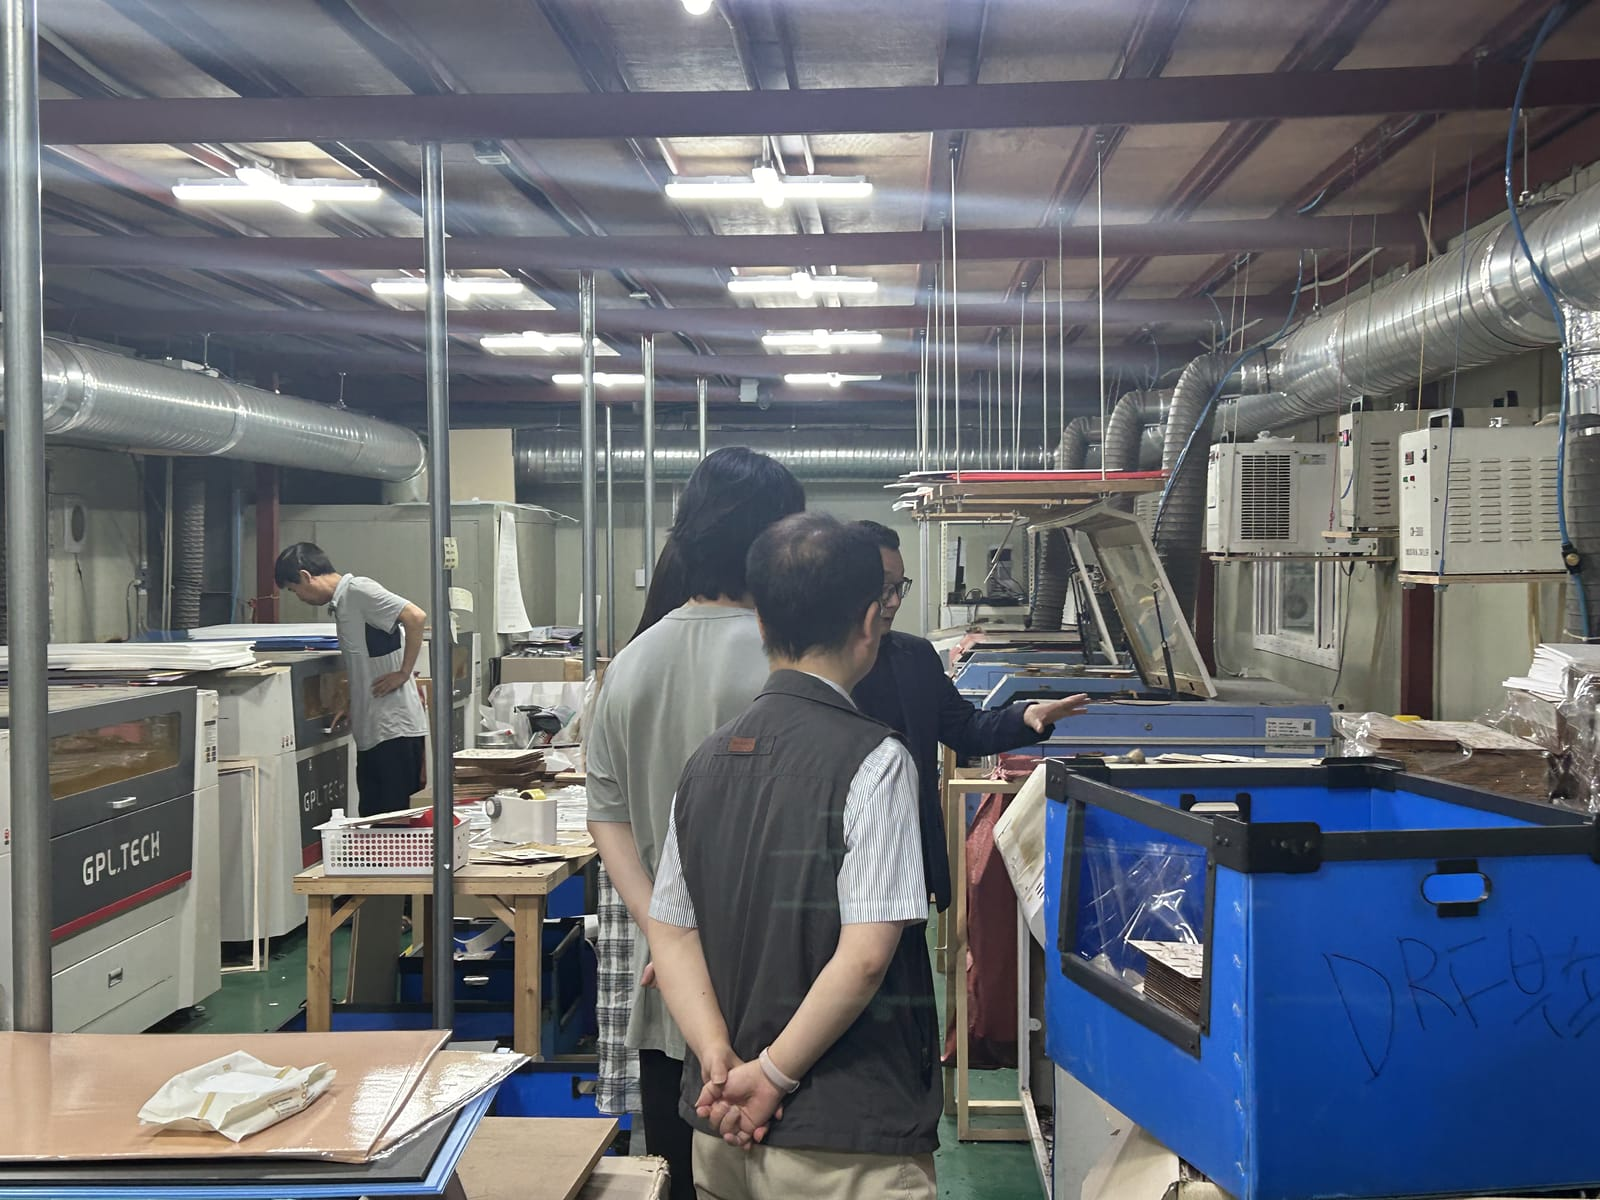
\includegraphics[width=\linewidth, height=3.6cm, keepaspectratio]{../img/2일차_IMG_2964.jpg}
    \caption{커팅기 작동 참관}
  \end{subfigure}
  \caption{2일차 — 제작 협력업체(D-RISE) 레이저 커팅 공장 생산 공정 견학}
\end{figure}

%% ---- 사진: 2일차 물류·시연 4장 ----
\begin{figure}[H]\centering
  \begin{subfigure}{0.24\linewidth}\centering
    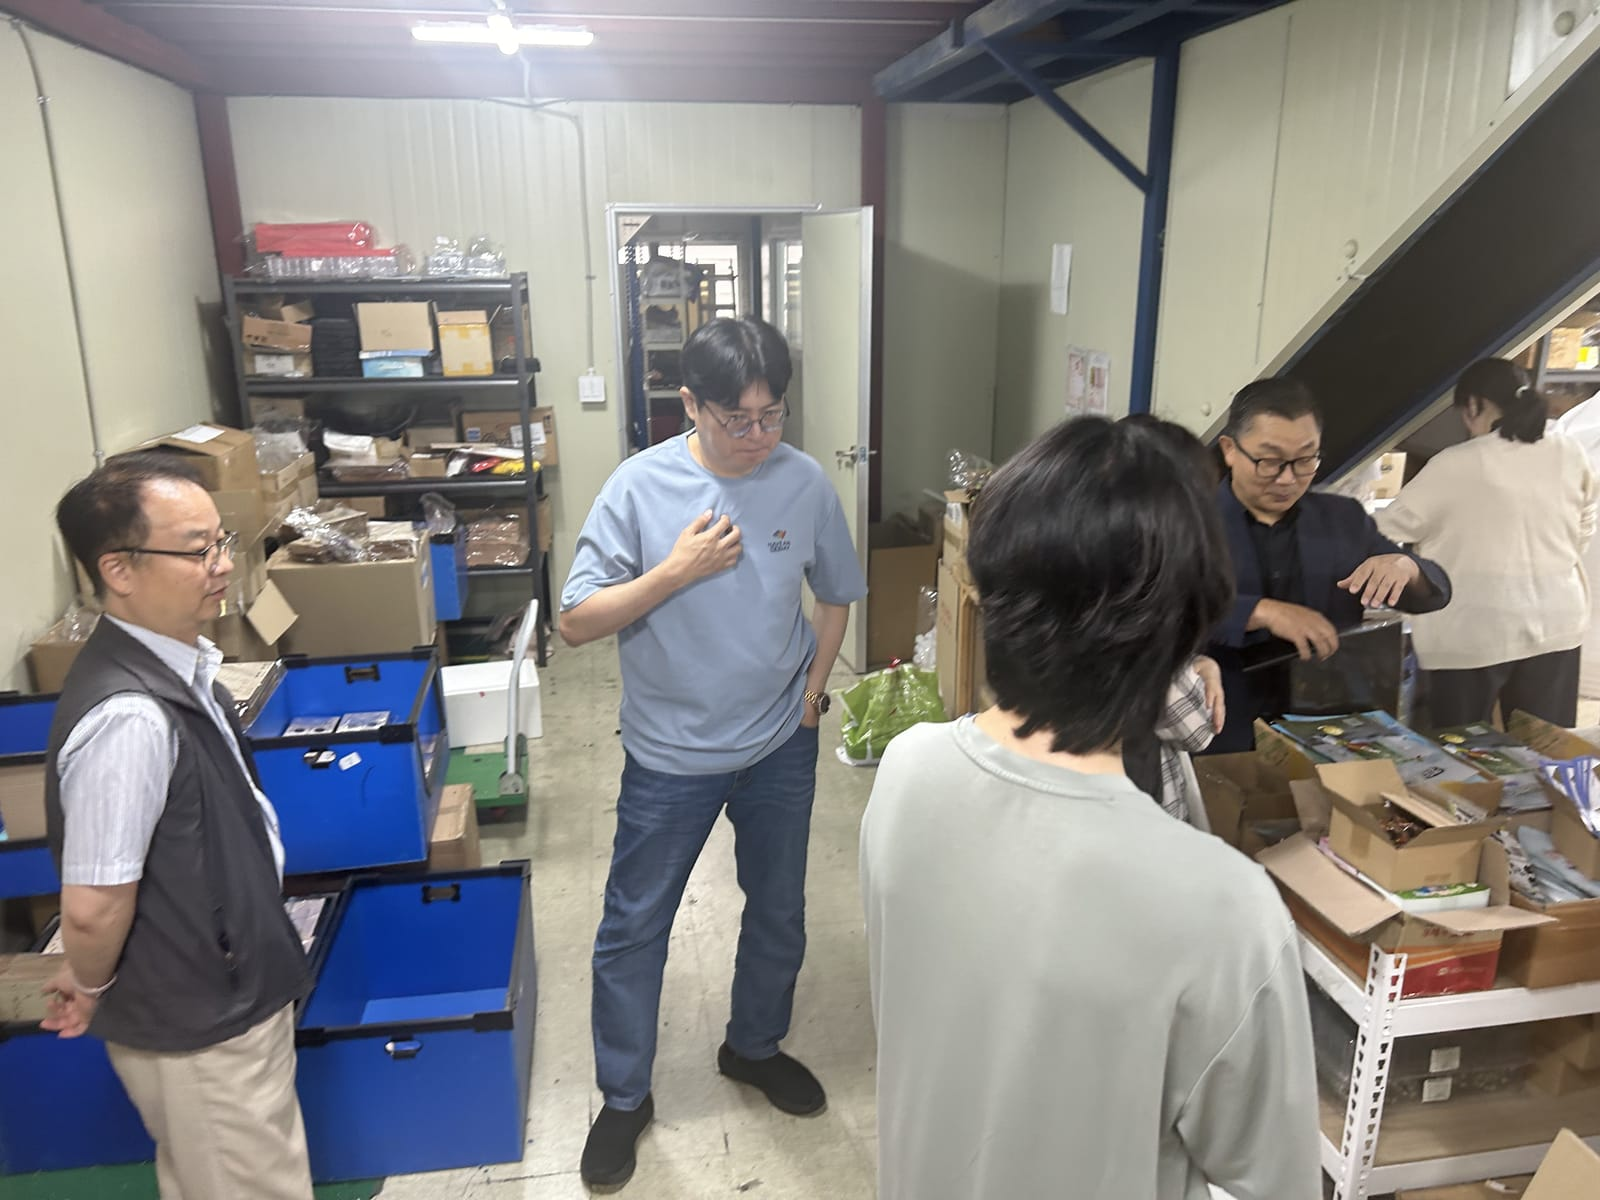
\includegraphics[width=\linewidth, height=3.6cm, keepaspectratio]{../img/2일차_IMG_2965.jpg}
    \caption{창고 재고$\cdot$물류 (10:47)}
  \end{subfigure}\hfill
  \begin{subfigure}{0.24\linewidth}\centering
    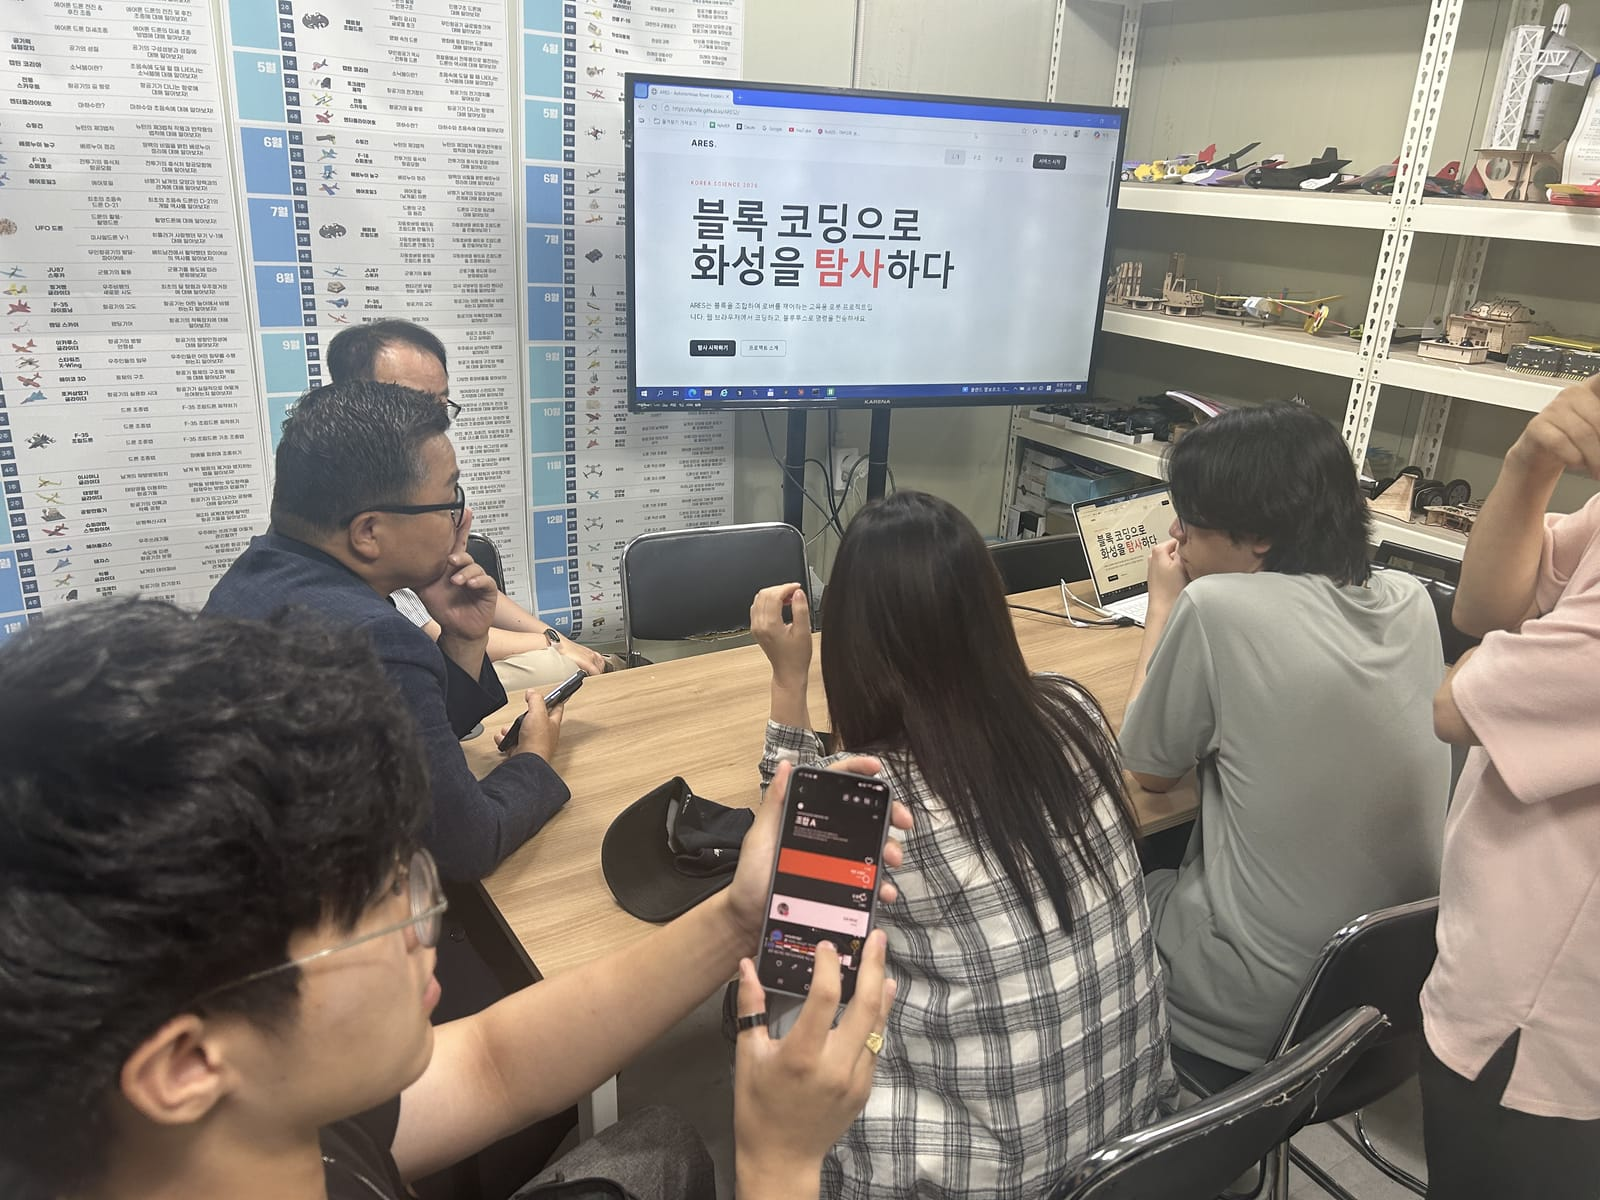
\includegraphics[width=\linewidth, height=3.6cm, keepaspectratio]{../img/2일차_IMG_2966.jpg}
    \caption{웹 랜딩 시연 (11:10)}
  \end{subfigure}\hfill
  \begin{subfigure}{0.24\linewidth}\centering
    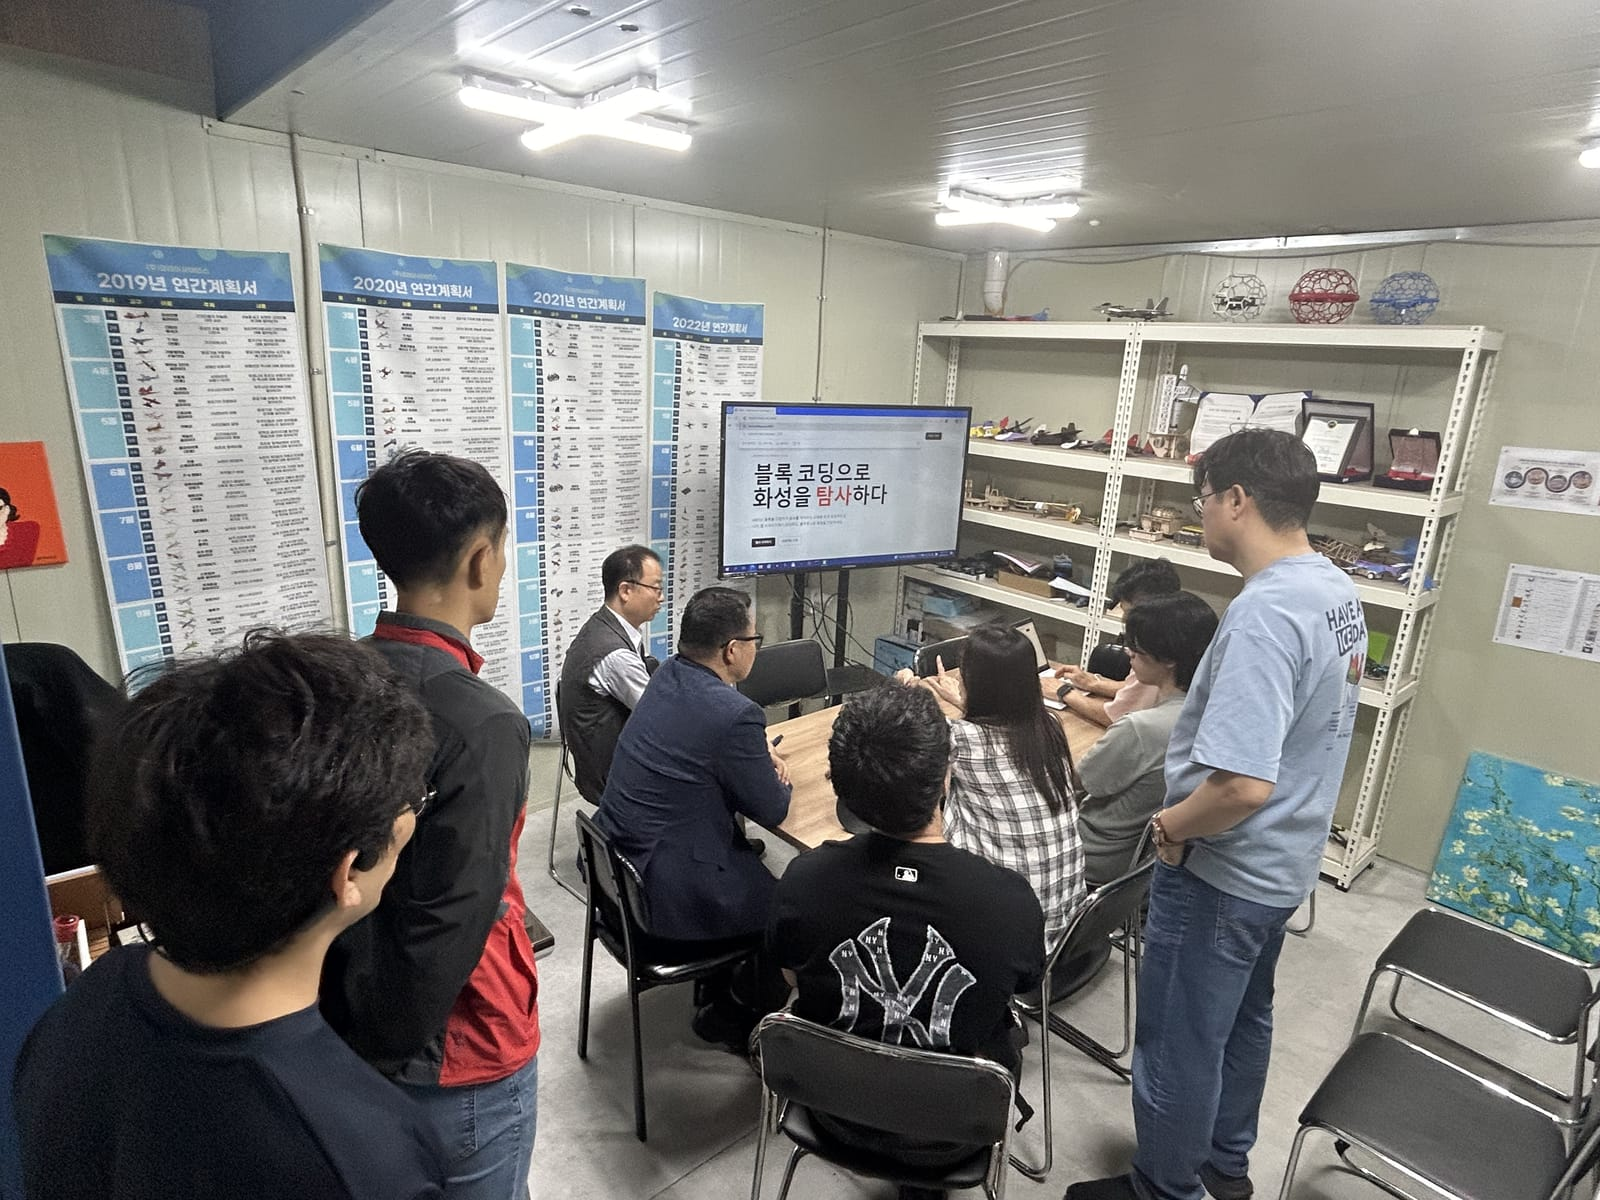
\includegraphics[width=\linewidth, height=3.6cm, keepaspectratio]{../img/2일차_IMG_2967.jpg}
    \caption{웹 서비스 발표}
  \end{subfigure}\hfill
  \begin{subfigure}{0.24\linewidth}\centering
    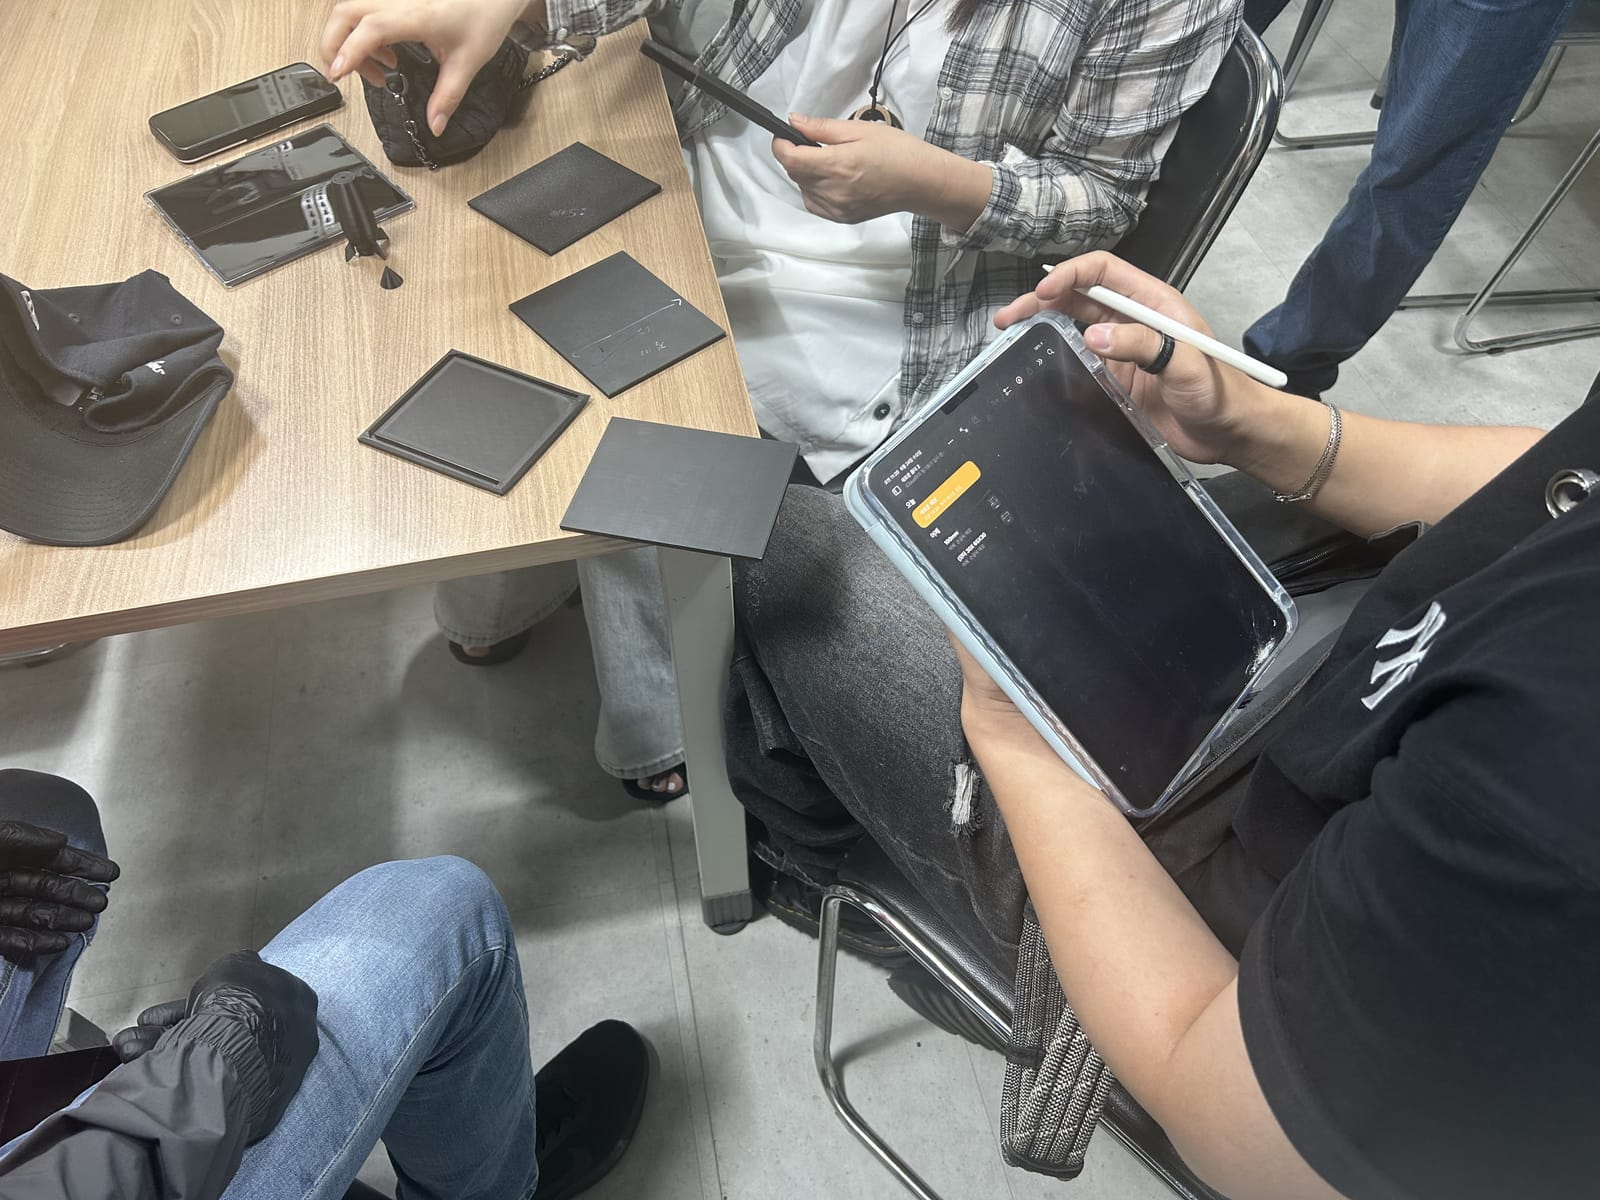
\includegraphics[width=\linewidth, height=3.6cm, keepaspectratio]{../img/2일차_IMG_2968.jpg}
    \caption{부품$\cdot$앱 통합 검토 (11:20)}
  \end{subfigure}
  \caption{2일차 — 창고 물류 협의와 회의실 웹 서비스 시연$\cdot$리뷰}
\end{figure}

% ============================================================
\section{3일차 — 개발 지속 · 디자인 프로토타입 제작}
\textit{2026.06.25 (수) · 10:00\,--\,17:00 KST}

\begin{summarybox}
컴퓨터실로 복귀해 개발을 이어갔다. 통합$\cdot$검증 작업과 함께 1차 Refactoring
계획을 수립하고, 자체 설계 디자인을 3D 프린터로 출력해 프로토타입을 점검하며
추가 디자인 계획을 세웠다.
\end{summarybox}

\subsection{주요 업무 — 1차 Refactoring 계획 수립}
지나치게 큰 함수$\cdot$파일로 분석이 어려운 소스를 기능 단위로 분할하기 위한
\textbf{「1차 Refactoring 계획」}을 수립했다. \emph{동작 보존(behavior-preserving)}을
원칙으로, 비대 지점을 네 가지 문제 유형으로 분류하고 6단계 로드맵을
도출했다~\cite{fowler2018refactoring, martin2008cleancode}. 전문은 부록~\ref{app:refactor1}.

%% ---- 부록 발췌 2: 진단표 ----
\begin{table}[H]\centering\small
\caption{비대 지점 진단 (상위 4건, 부록~\ref{app:refactor1} 발췌)}
\renewcommand{\arraystretch}{1.2}
\begin{tabularx}{\linewidth}{@{}>{\ttfamily\footnotesize}l c L{0.5\linewidth}@{}}
\toprule
\sffamily 파일 & \sffamily 줄수 & \sffamily 핵심 문제 \\
\midrule
Web/simulation.js     & 2333 & 거대 클로저 2개에 10개 서브시스템이 엉킴 \\
Web/main.js           & 1051 & 한 함수가 미션/저장/예제/AI/대시보드를 전부 처리 \\
Web/dashboard.html    & 828  & HTML 안에 CSS 362 + JS 385 인라인 \\
Pico/process\_data.py & 653  & 거대 if/elif 디스패처 + 30개 핸들러 한 클래스 \\
\bottomrule
\end{tabularx}
\end{table}

\noindent 위 비대 지점은 네 유형으로 분류된다 ---
\chip{A · 거대 클로저}~\chip{B · 거대 디스패처}~\chip{C · 데이터 덩어리}~\chip{D · 인라인 자산}.
각 유형의 대응 패턴과 6단계 로드맵은 부록~\ref{app:refactor1}을 참조한다.

\subsection{주요 업무 — 디자인 프로토타입 출력 \& 추가 디자인 계획}
자체 설계한 디자인을 \textbf{3D 프린터로 출력}해 실물 프로토타입의 형상$\cdot$조립성을
검증하고, \textbf{Autodesk 3ds Max로 후속 디자인을 모델링}하며 추가 디자인 계획을
수립했다. 부저 스피커 베이스(‘코리아사이언스’ 각인)$\cdot$로켓 노즈콘$\cdot$LED 마운트
등 자체 제작 부품을 출력해 컨트롤러$\cdot$모터와 함께 배치하고 조립성을 점검했다.

%% ---- 사진: 3일차 4장 ----
\begin{figure}[H]\centering
  \begin{subfigure}{0.24\linewidth}\centering
    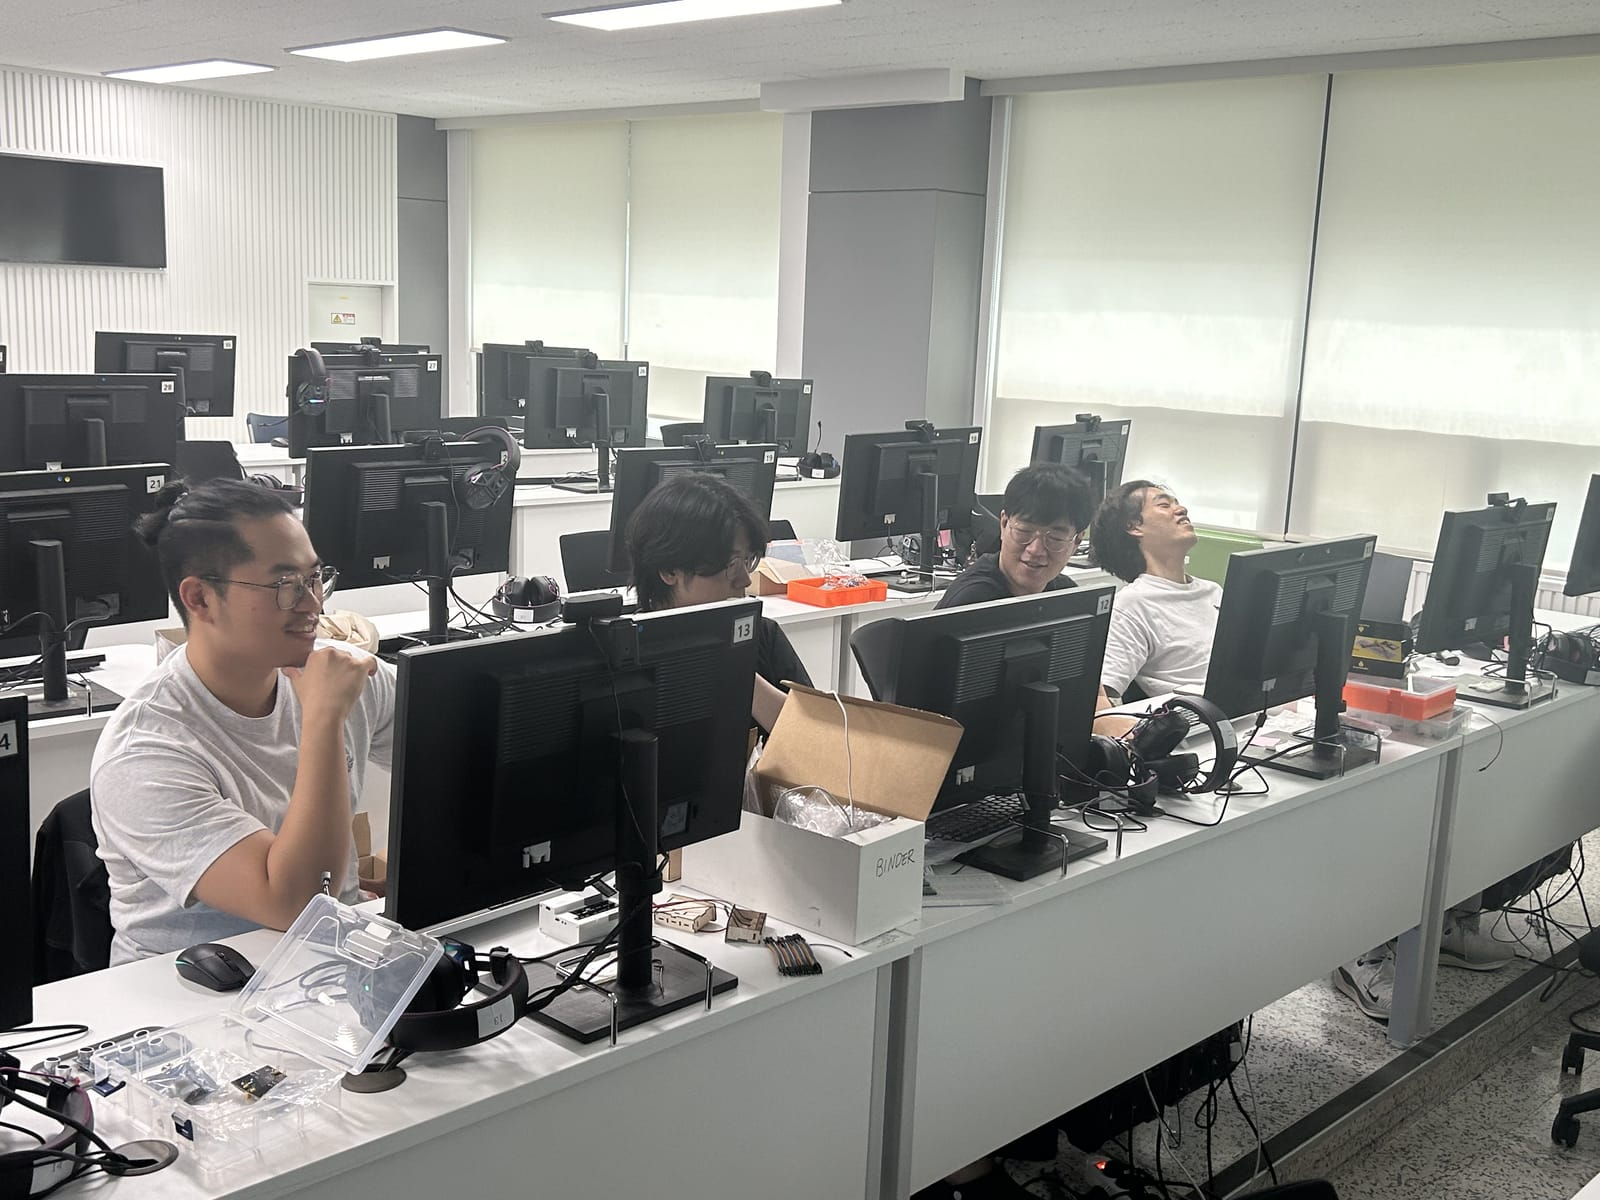
\includegraphics[width=\linewidth, height=3.6cm, keepaspectratio]{../img/3일차_IMG_2998.jpg}
    \caption{개발 지속 (11:19)}
  \end{subfigure}\hfill
  \begin{subfigure}{0.24\linewidth}\centering
    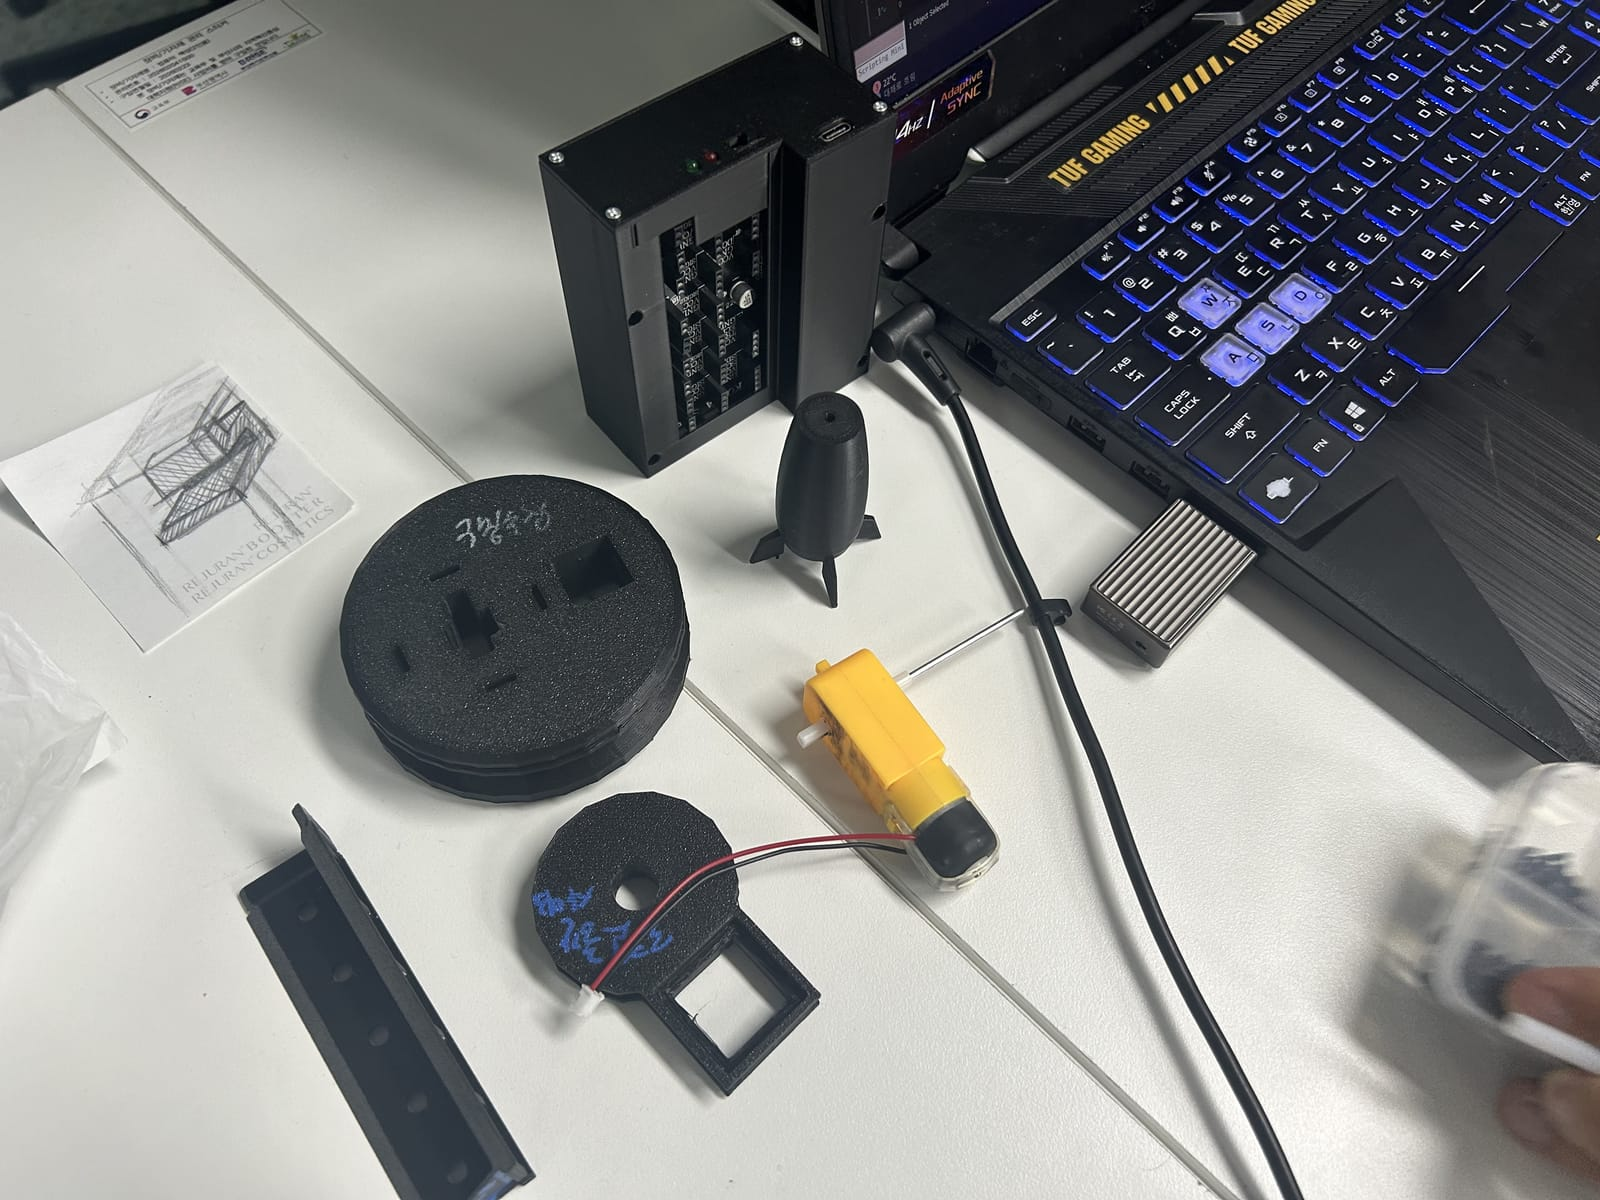
\includegraphics[width=\linewidth, height=3.6cm, keepaspectratio]{../img/3일차_IMG_2999.jpg}
    \caption{3D 프린팅 프로토타입}
  \end{subfigure}\hfill
  \begin{subfigure}{0.24\linewidth}\centering
    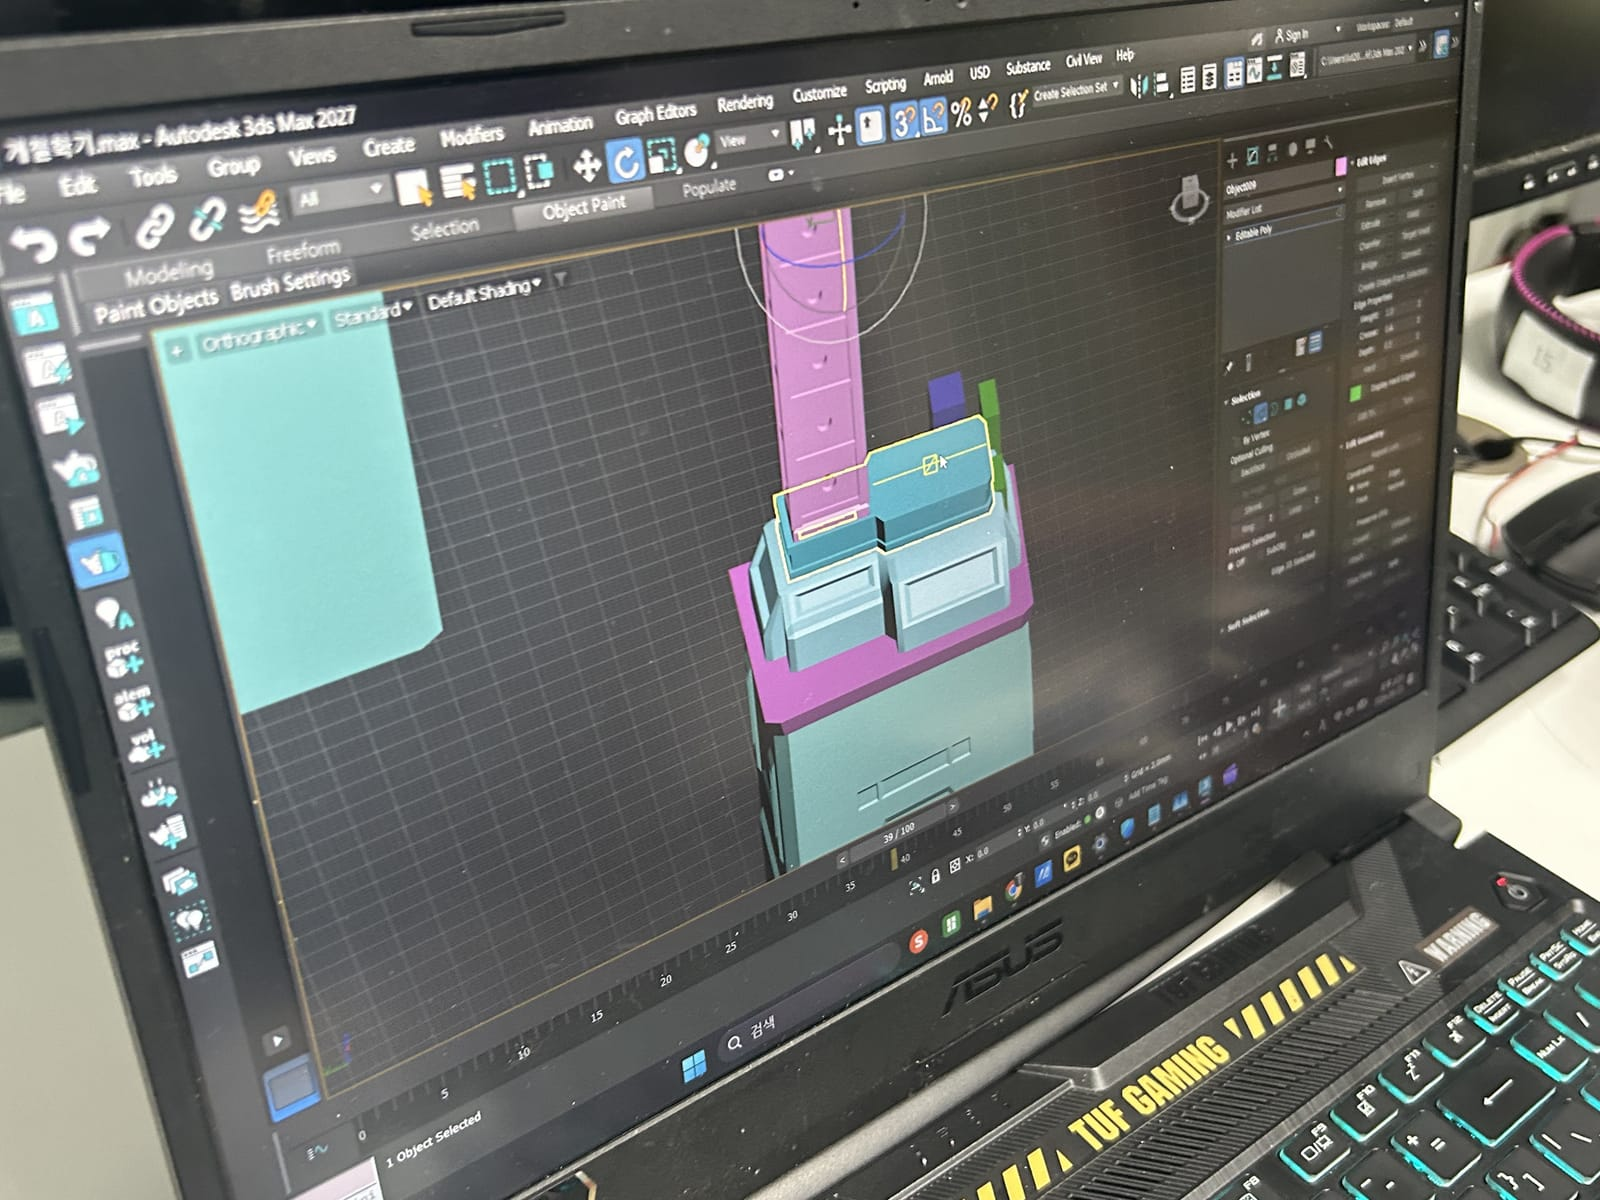
\includegraphics[width=\linewidth, height=3.6cm, keepaspectratio]{../img/3일차_IMG_3001.jpg}
    \caption{3ds Max 모델링}
  \end{subfigure}\hfill
  \begin{subfigure}{0.24\linewidth}\centering
    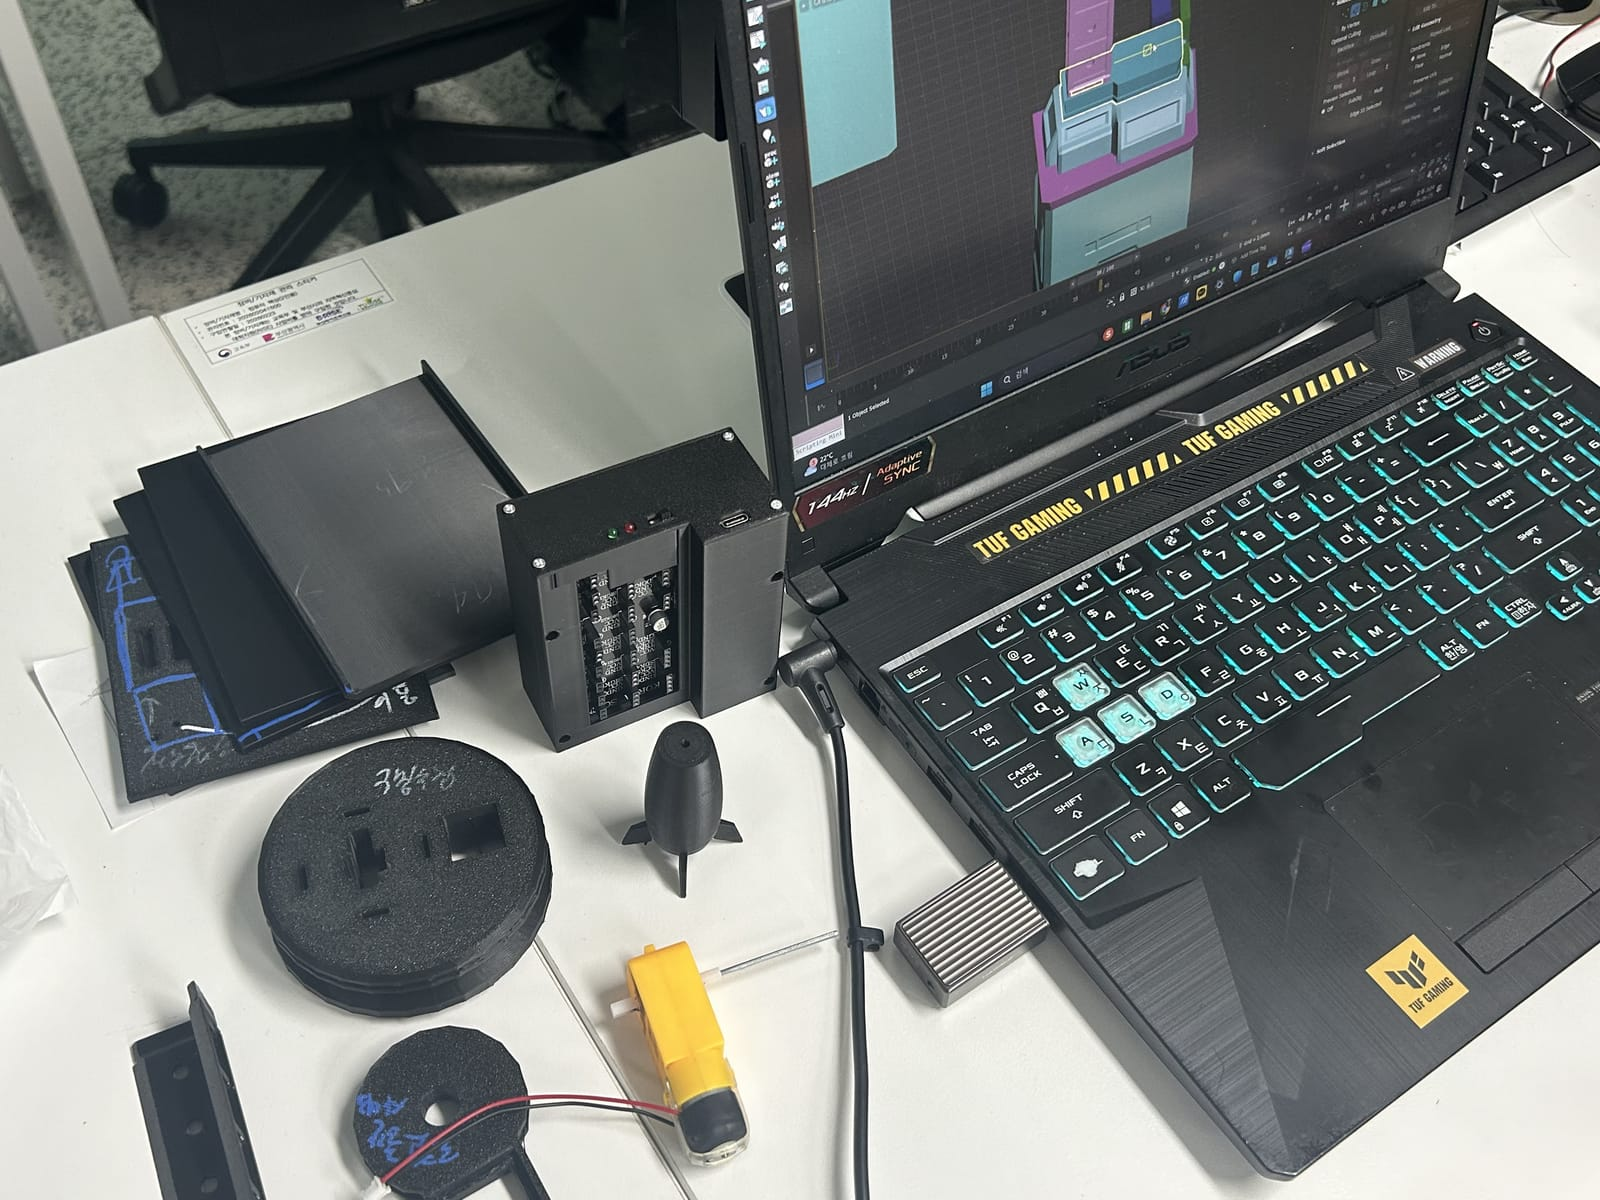
\includegraphics[width=\linewidth, height=3.6cm, keepaspectratio]{../img/3일차_IMG_3002.jpg}
    \caption{출력물$\cdot$모델 대조 (15:24)}
  \end{subfigure}
  \caption{3일차 — 디자인 프로토타입 출력과 3ds Max 후속 모델링$\cdot$검토}
\end{figure}

% ============================================================
\section{4일차 — 1차시 운영 점검 · 통합 개발}
\textit{2026.06.26 (목) · 10:00\,--\,17:00 KST}

\begin{summarybox}
수업 적용을 앞두고 1차시 운영을 점검했다. 제품 동작과 교구 학습 진도를
확인하고, 웹 인터페이스와 WebGL 3D 시뮬레이션을 점검해 「2차 Refactoring 계획」을
수립했다. 또한 조립형 모델 시작품을 제작하고, 시뮬레이션$\cdot$피코 펌웨어$\cdot$웹
인터페이스 세 트랙의 개발을 진행했다.
\end{summarybox}

\subsection{주요 업무 — 1차시 운영 점검 (제품 동작 · 교구 학습)}
ARES 키트의 실제 수업 적용을 앞두고 1차시 운영을 점검했다. 조립된 4륜 로버와
3D 프린팅 컨트롤러 케이스(전원 LED 점등)를 연결하고 방향 표시 디스크 교구와
함께 제품 동작을 확인했으며, 모니터에 학습 콘텐츠(‘화성 탐사선 코딩 여정’)를
띄워 차시별 교구 학습 진도를 점검했다.

\begin{figure}[H]\centering
  \begin{subfigure}{0.46\linewidth}\centering
    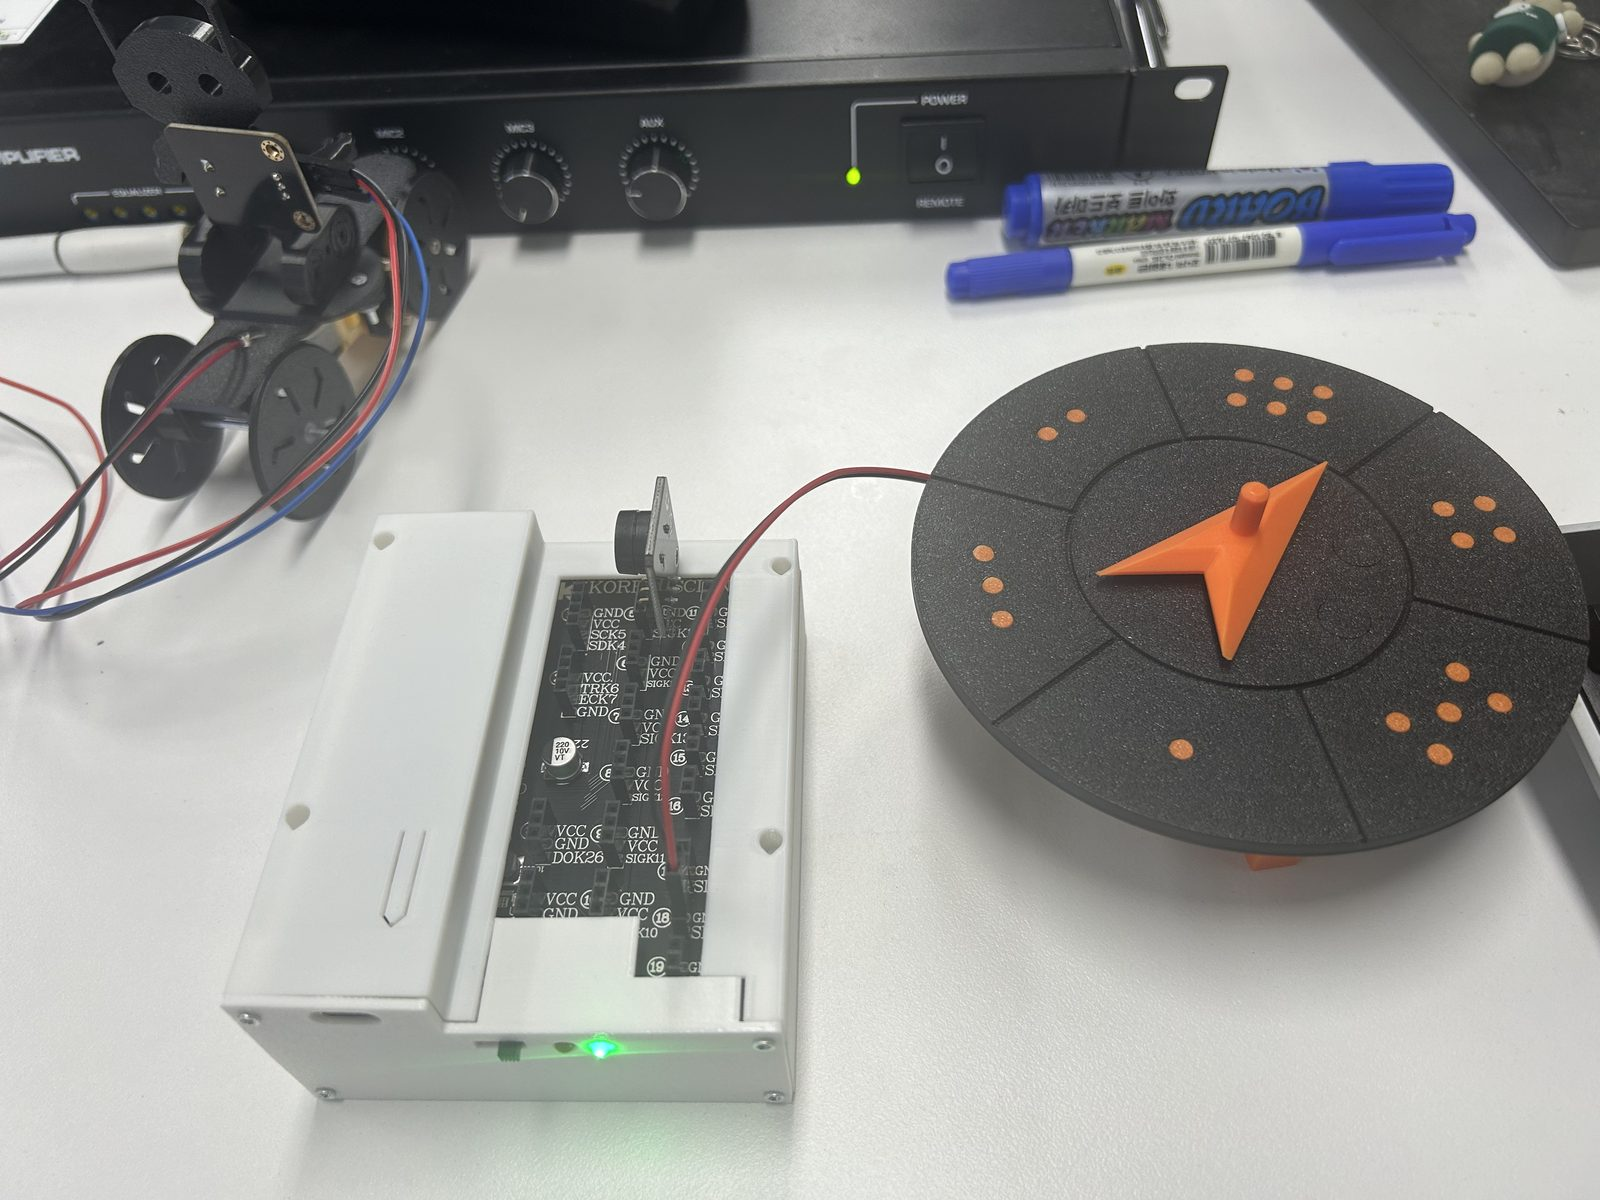
\includegraphics[width=\linewidth, height=5.0cm, keepaspectratio]{../img/4일차_1차시_제품동작확인.jpg}
    \caption{제품 동작 확인 — 로버$\cdot$컨트롤러$\cdot$방향 디스크 교구 (11:33)}
  \end{subfigure}\hfill
  \begin{subfigure}{0.46\linewidth}\centering
    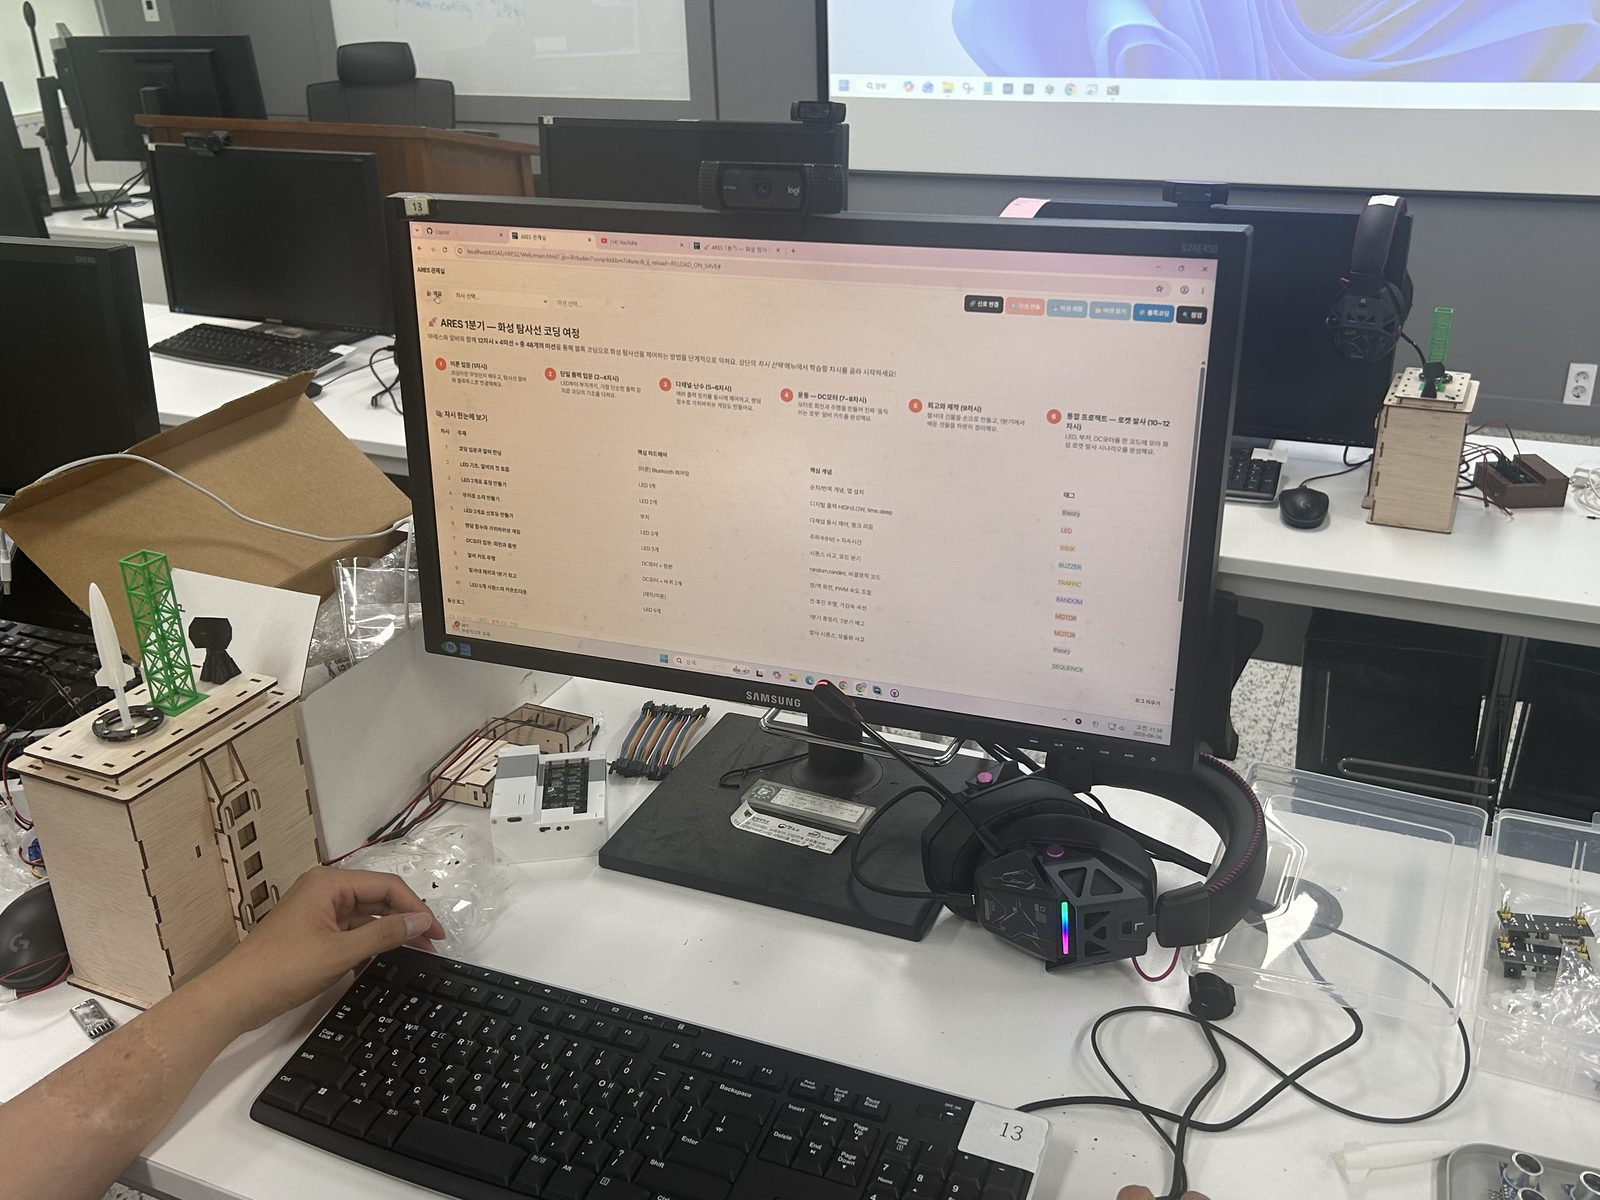
\includegraphics[width=\linewidth, height=5.0cm, keepaspectratio]{../img/4일차_교구학습진도.jpg}
    \caption{교구 학습 진도 점검 — 학습 콘텐츠$\cdot$발사대 모형 (11:42)}
  \end{subfigure}
  \caption{4일차 — 1차시 운영 점검(제품 동작$\cdot$교구 학습)}
\end{figure}

\subsection{주요 업무 — 웹 인터페이스·3D 시뮬레이션 점검 \& 2차 Refactoring 계획}
ARES 웹 서비스의 인터페이스와 WebGL 3D 시뮬레이션~\cite{threejs, webgl}을 팀이
함께 점검하고, 그 결과를 바탕으로 시뮬레이터$\cdot$피코+블록코딩$\cdot$웹 인터페이스
세 트랙의 \textbf{「2차 Refactoring 계획」}을 수립했다. 전문은 부록~\ref{app:refactor2}.

\begin{figure}[H]\centering
  \begin{subfigure}{0.32\linewidth}\centering
    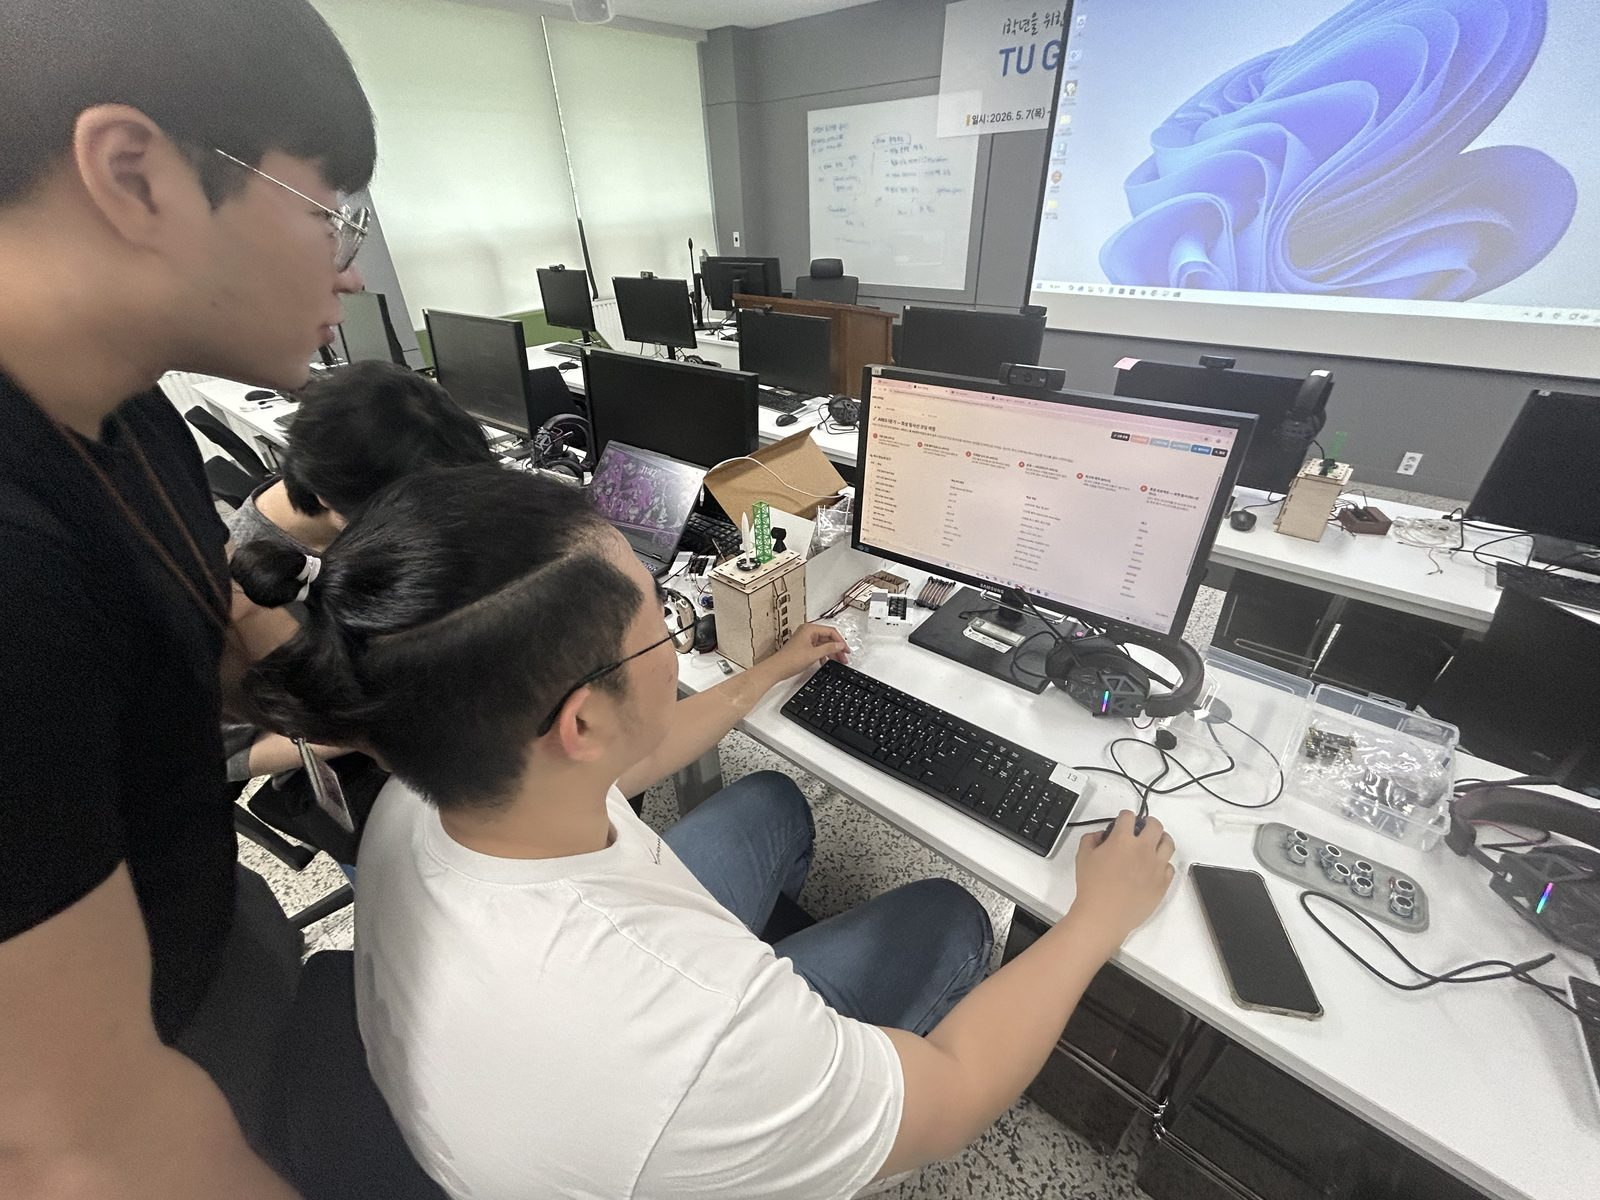
\includegraphics[width=\linewidth, height=4.0cm, keepaspectratio]{../img/4일차_웹인터페이스점검.jpg}
    \caption{웹 인터페이스 점검 (11:42)}
  \end{subfigure}\hfill
  \begin{subfigure}{0.32\linewidth}\centering
    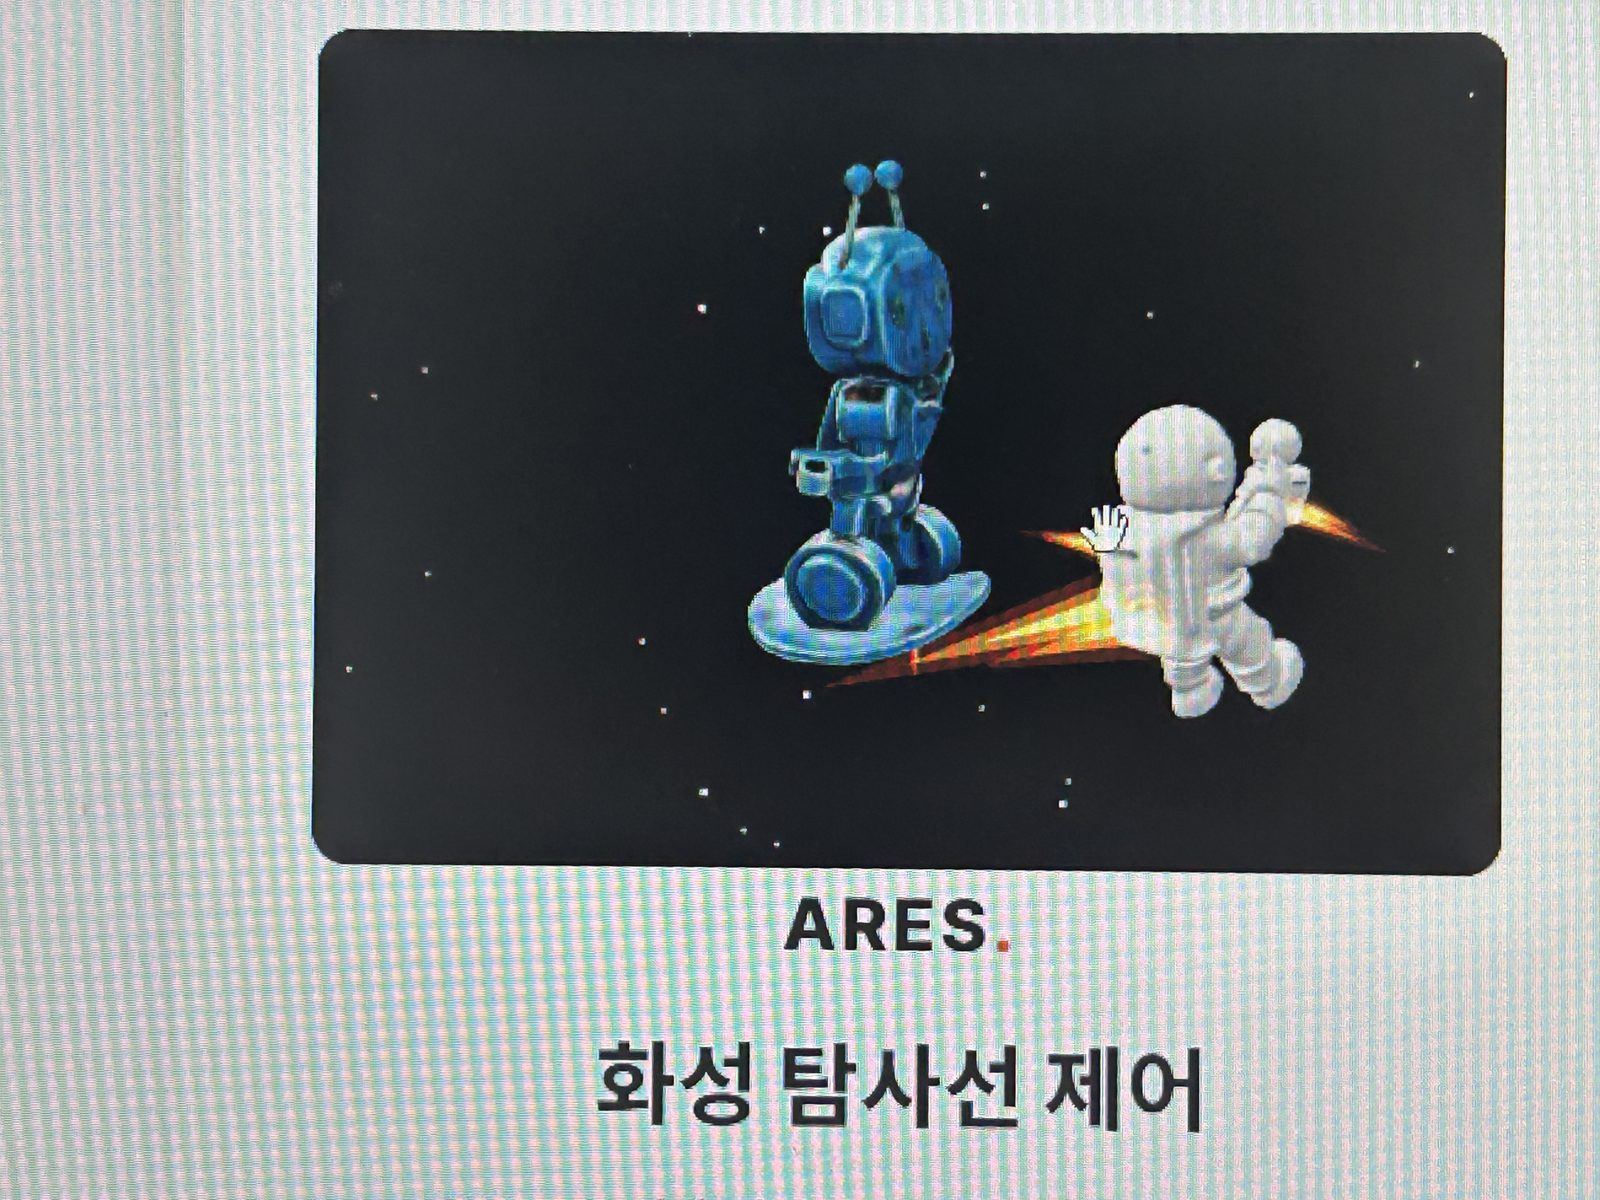
\includegraphics[width=\linewidth, height=4.0cm, keepaspectratio]{../img/4일차_시뮬레이션점검.jpg}
    \caption{WebGL 3D 시뮬레이션 (13:38)}
  \end{subfigure}\hfill
  \begin{subfigure}{0.32\linewidth}\centering
    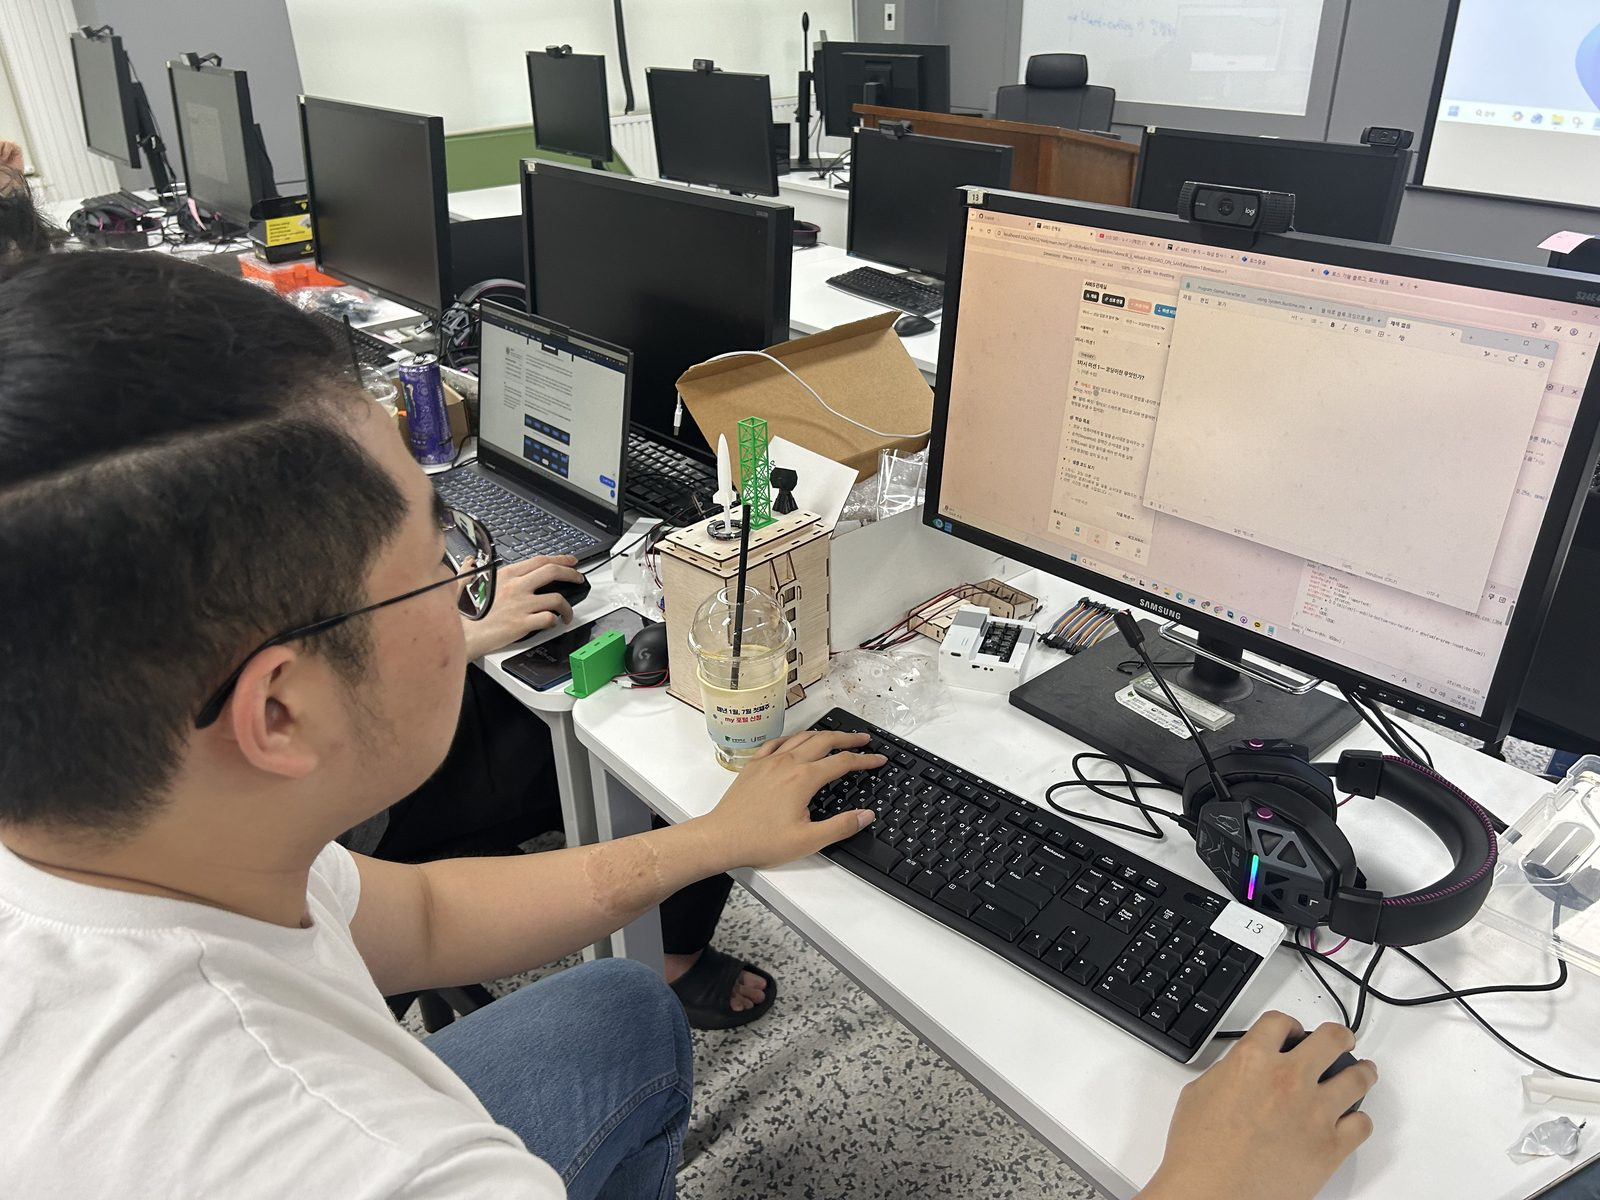
\includegraphics[width=\linewidth, height=4.0cm, keepaspectratio]{../img/4일차_인터페이스개선계획수립.jpg}
    \caption{개선 계획(2차 Refactoring) 수립 (13:35)}
  \end{subfigure}
  \caption{4일차 — 웹 인터페이스$\cdot$3D 시뮬레이션 점검과 2차 Refactoring 계획 수립}
\end{figure}

\subsection{주요 업무 — 조립형 모델 시작품 제작}
최종 제품의 \textbf{배선 조립}과 \textbf{외형 조립}이 쉬워지도록, 본체$\cdot$외형 패널$\cdot$상단
발사대 모듈로 분해$\cdot$결합되는 \textbf{조립형 모델 시작품}을 3D 프린팅으로
제작했다. 내부 구동부와 배선을 먼저 배치한 뒤 측면 외형 패널과 상단 모듈을
끼워 맞추는 \emph{모듈형 결합 구조}로, 양산 시 조립$\cdot$점검$\cdot$유지보수가 용이한지를
실물로 검증했다. 디자인 부품 시제품은 Bambu Lab 3D 프린터로 출력했다.

\begin{figure}[H]\centering
  \begin{subfigure}{0.19\linewidth}\centering
    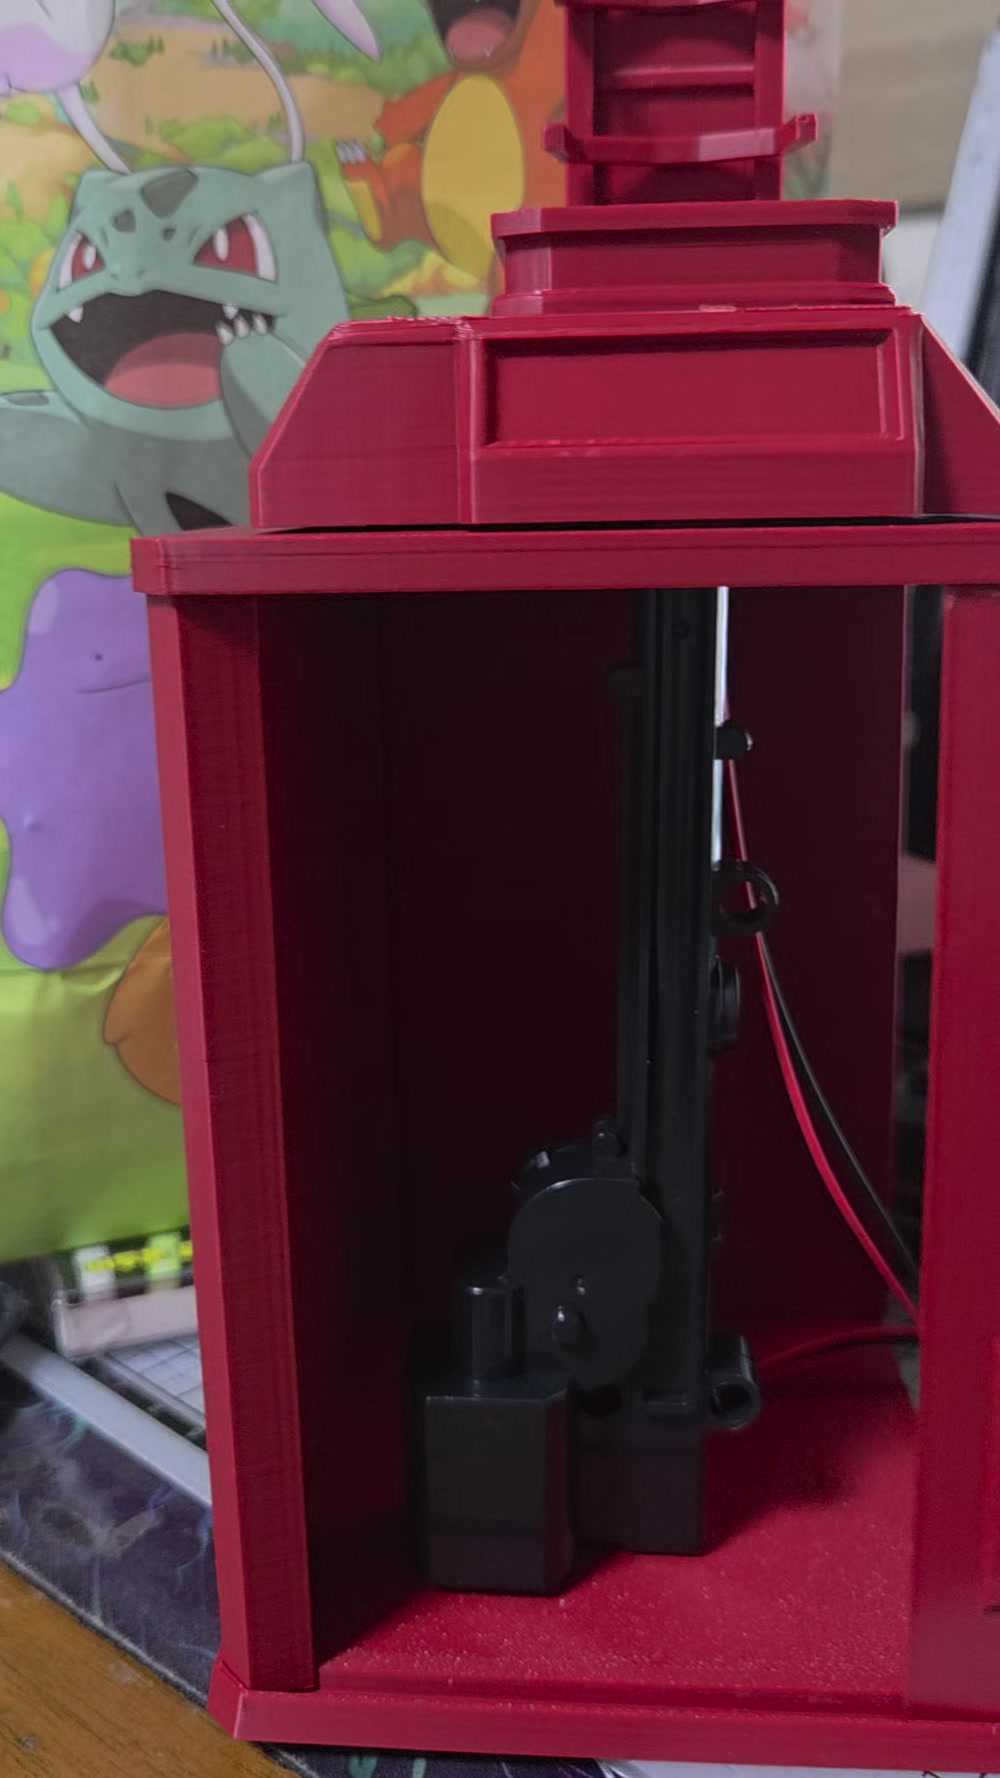
\includegraphics[width=\linewidth, height=3.8cm, keepaspectratio]{../img/4일차_조립형모델_내부배선.jpg}
    \caption{\textcircled{1} 내부 배선}
  \end{subfigure}\hfill
  \begin{subfigure}{0.19\linewidth}\centering
    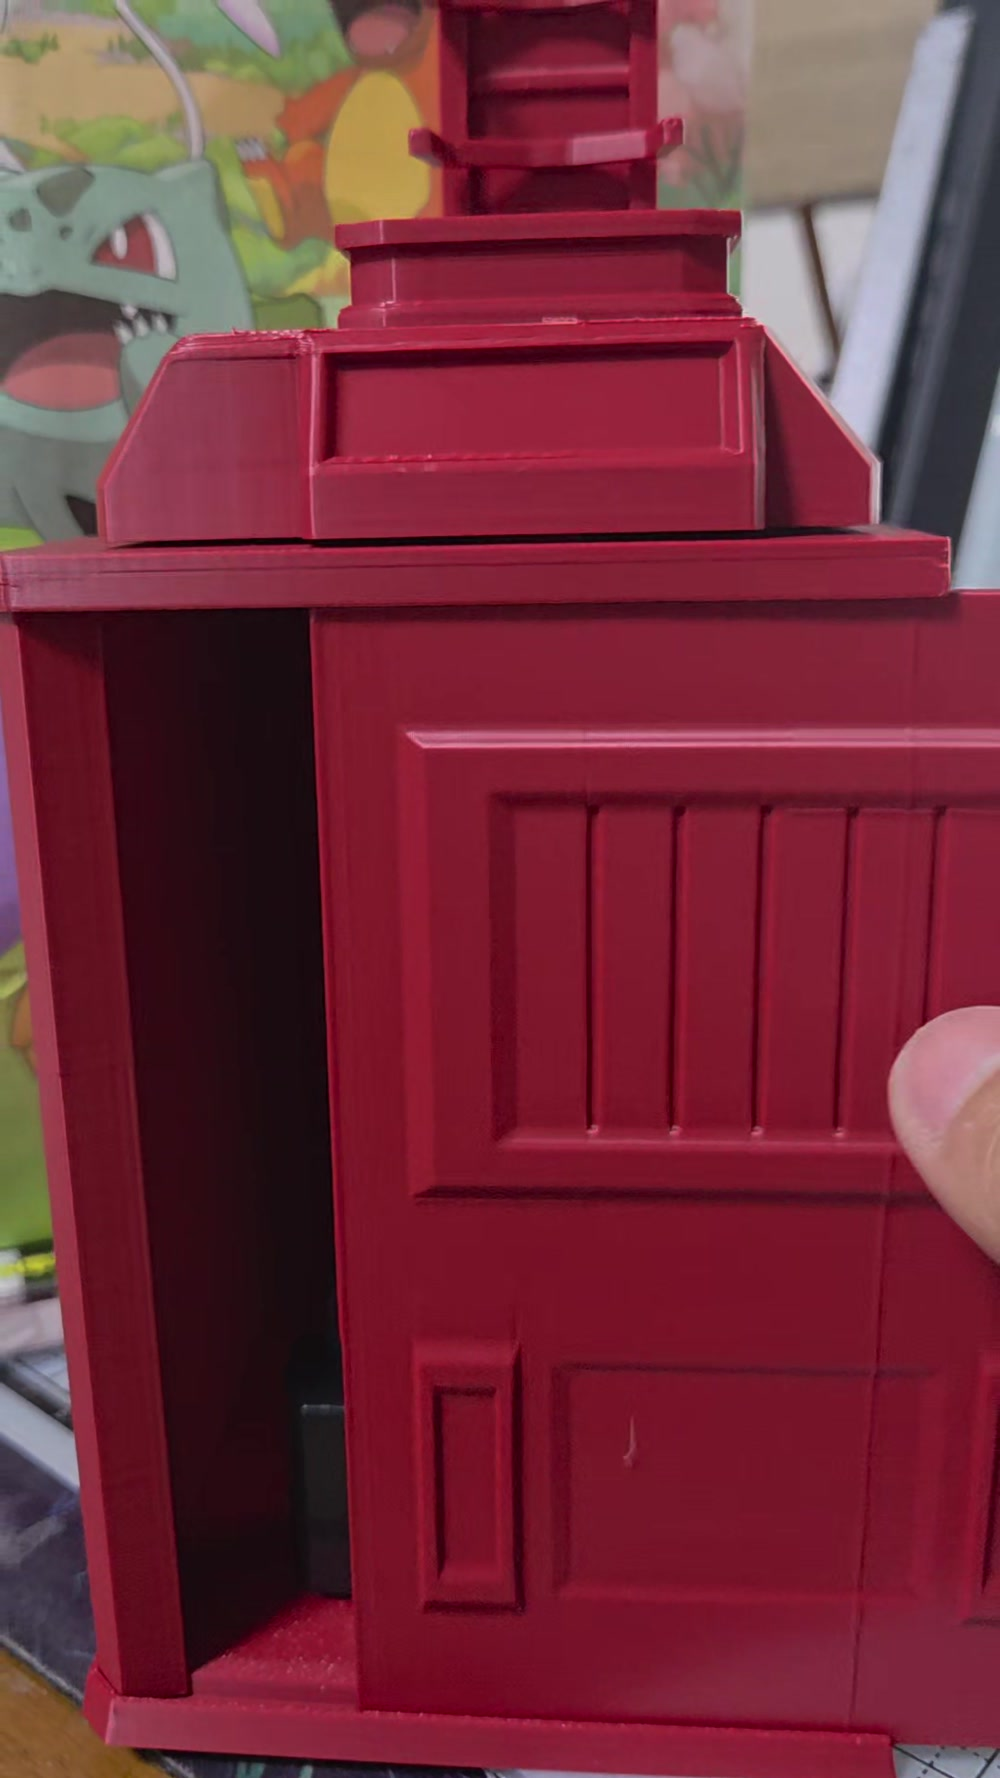
\includegraphics[width=\linewidth, height=3.8cm, keepaspectratio]{../img/4일차_조립형모델_외형패널.jpg}
    \caption{\textcircled{2} 외형 패널}
  \end{subfigure}\hfill
  \begin{subfigure}{0.19\linewidth}\centering
    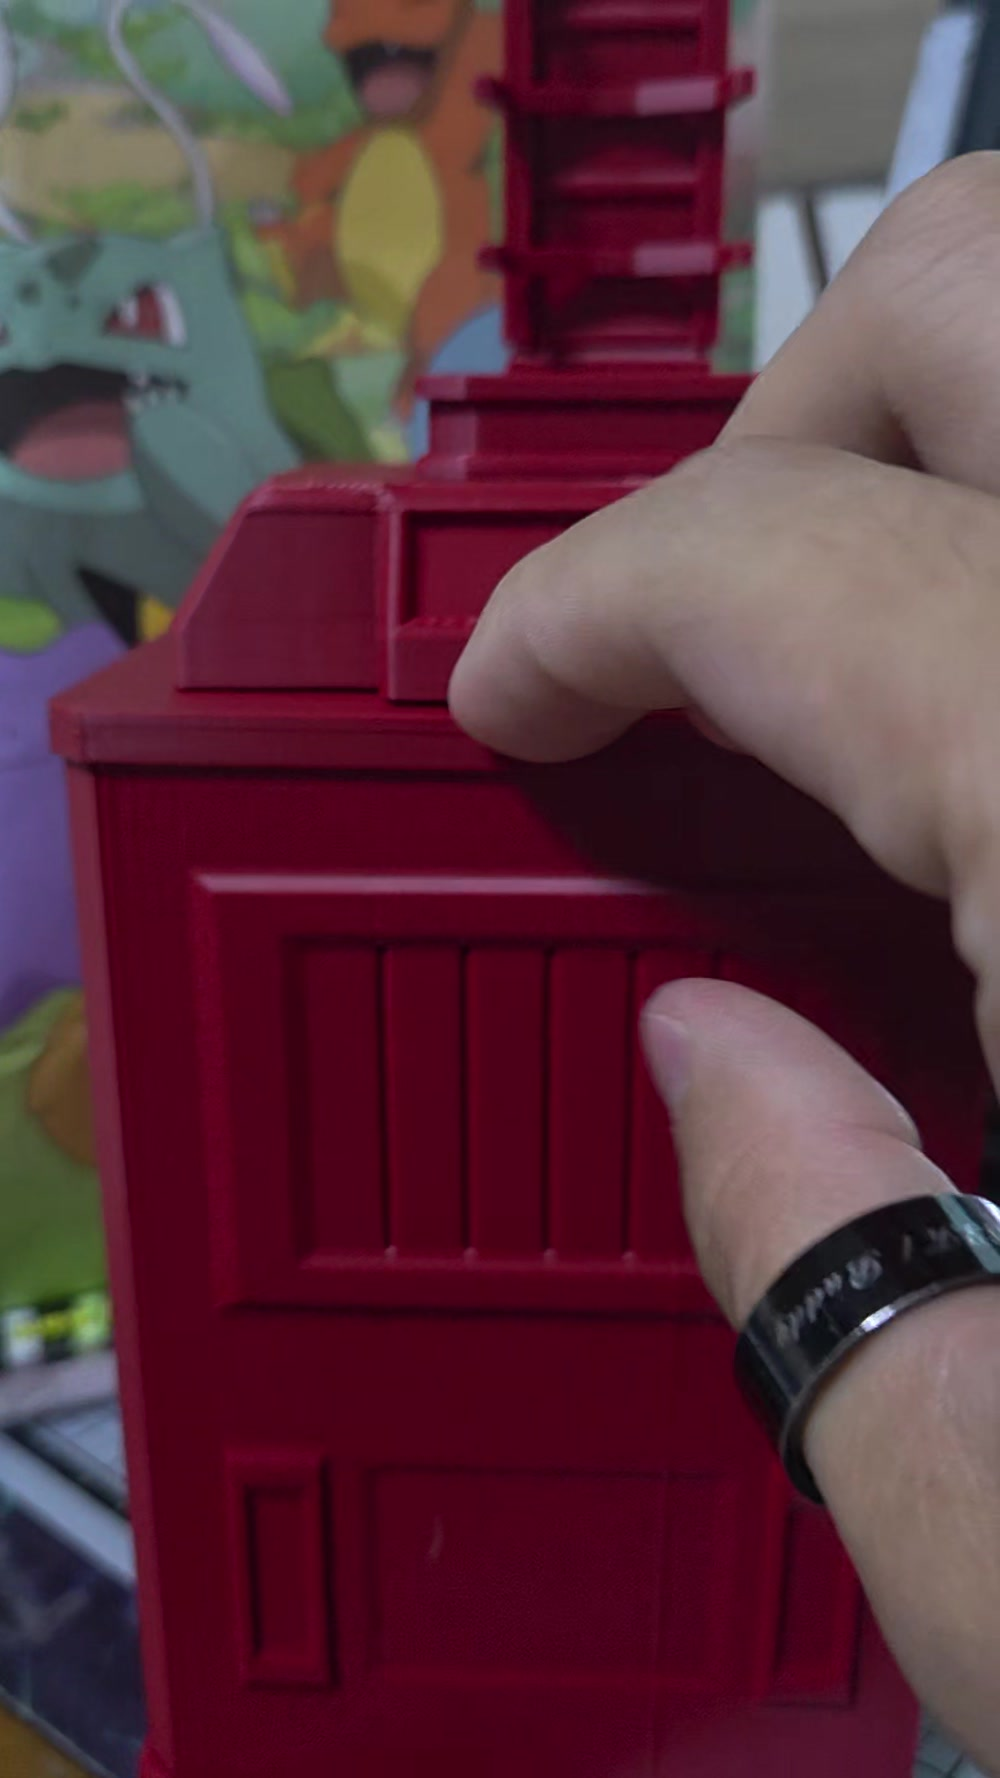
\includegraphics[width=\linewidth, height=3.8cm, keepaspectratio]{../img/4일차_조립형모델_상단모듈.jpg}
    \caption{\textcircled{3} 상단 모듈}
  \end{subfigure}\hfill
  \begin{subfigure}{0.19\linewidth}\centering
    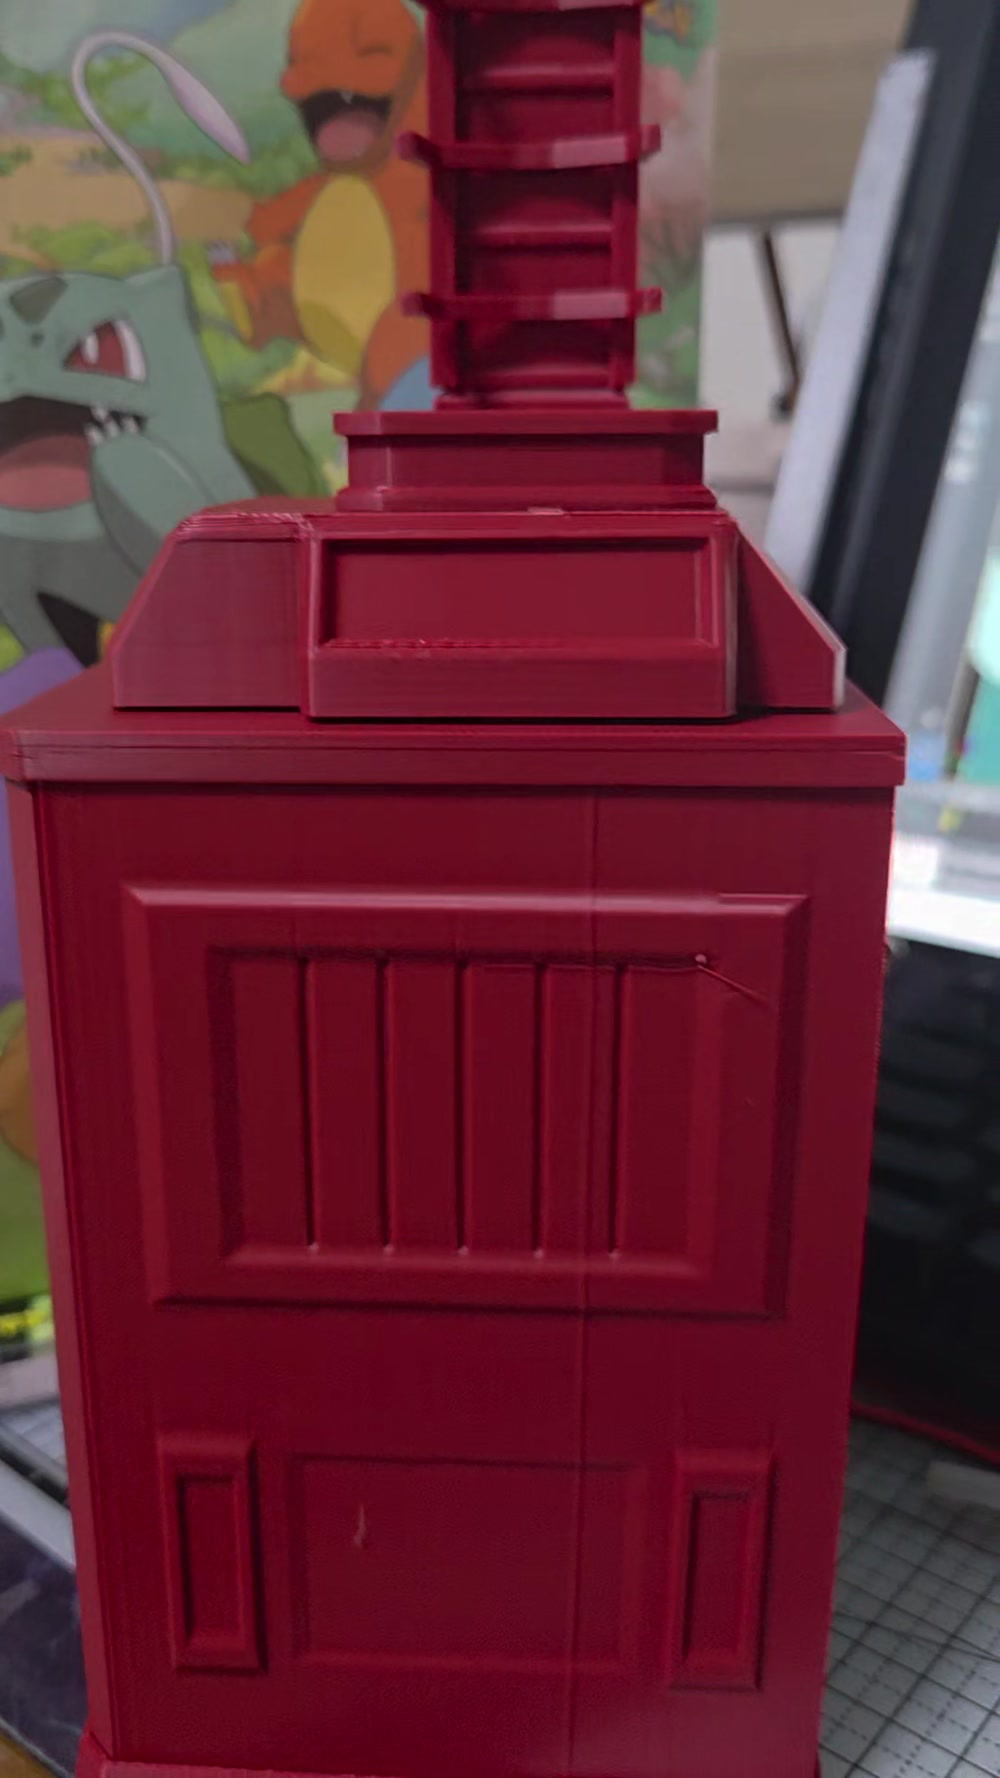
\includegraphics[width=\linewidth, height=3.8cm, keepaspectratio]{../img/4일차_조립형모델_완성.jpg}
    \caption{\textcircled{4} 완성}
  \end{subfigure}\hfill
  \begin{subfigure}{0.19\linewidth}\centering
    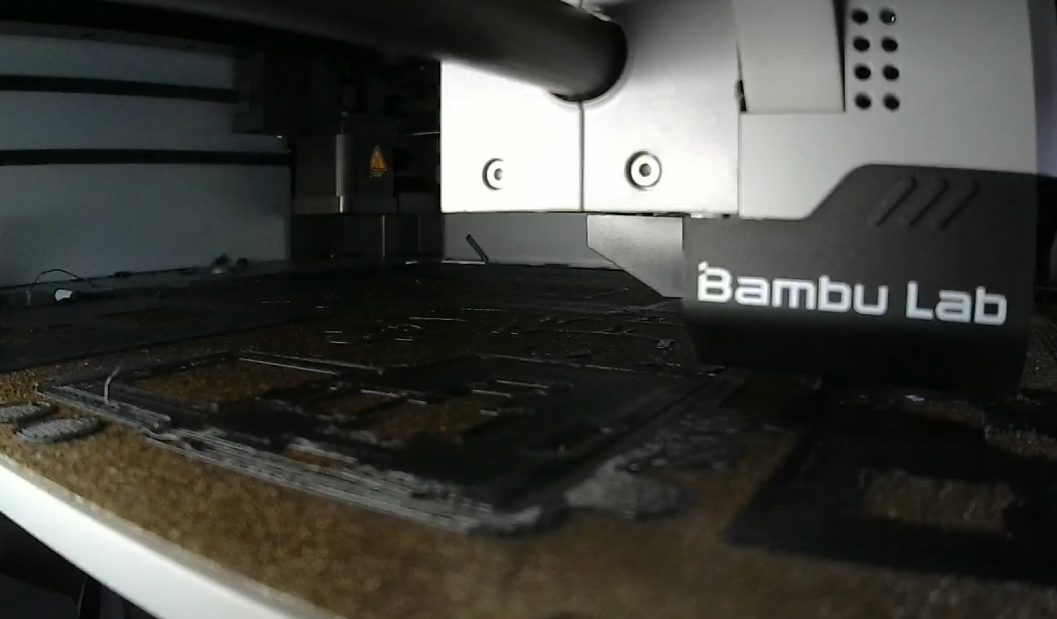
\includegraphics[width=\linewidth, height=3.8cm, keepaspectratio]{../img/4일차_시제품제작.jpg}
    \caption{시제품 출력}
  \end{subfigure}
  \caption{조립형 모델 시작품 — 분해 $\to$ 배선 $\to$ 외형 결합 $\to$ 완성(제작 영상 캡처)과 Bambu Lab 시제품 출력}
\end{figure}

\subsection{주요 업무 — 시뮬레이션 모듈 분할 리팩터링 (유형 A 실행)}
「2차 Refactoring 계획」의 첫 실행으로, 가장 비대했던 \code{simulation.js}(2,407줄)의
거대 클로저 \code{buildSim()}를 \emph{동작 보존} 원칙 아래 \textbf{공유 컨텍스트(ctx) +
서브시스템 모듈} 구조로 분해했다. 그 결과 \code{simulation.js}는 \textbf{372줄의 얇은
오케스트레이터}로 줄고, 기능은 \code{Web/Sim\_Parts/}~13개 모듈로 분리됐다.

%% ---- 부록 발췌 3: 시뮬 분할 ----
\begin{infobox}[title=부록 B 발췌 --- 유형 A 분할(시뮬레이터)]
\small
\code{buildSim()}에 묶여 있던 약 50개 상태를 \code{sim/context.js}(씬$\cdot$카메라$\cdot$렌더러$\cdot$ctx)로 끌어올리고, 기능을 \code{assets$\cdot$leds$\cdot$movement$\cdot$gun$\cdot$rocket$\cdot$traffic$\cdot$waves$\cdot$oled$\cdot$render$\cdot$audio$\cdot$dispatch$\cdot$topics} 모듈로 분리.
외부 인터페이스는 그대로라 \code{main.js}는 주석 1줄 외 변경 없음(2,407\,$\to$\,372줄).
음파 생성 보정$\cdot$중복 코드 정리 등 버그 수정 2건 병행.
\end{infobox}

\subsection{주요 업무 — 피코 펌웨어 설정 개편 \& 속도 기능}
펌웨어의 설정 체계를 \textbf{교사$\cdot$어린이가 메모장으로 직접 고치는 텍스트
설정}으로 바꾸고, 이동 블록에 \textbf{속도 조절}을 추가했다. 기존 \code{system.json}(JSON)을
주석$\cdot$섹션이 달린 \code{ModelFactorySetting.txt}로 대체해, 코드를 몰라도
속도$\cdot$핀$\cdot$모듈$\cdot$탭 이름을 직접 설정할 수 있게 했다.

%% ---- 부록 발췌 4: 명령 프로토콜 ----
\begin{table}[H]\centering\small
\caption{명령 프로토콜 발췌 — 속도 기능 추가 형식 (부록~\ref{app:code} 연계)}
\renewcommand{\arraystretch}{1.2}
\begin{tabularx}{\linewidth}{@{}>{\ttfamily\footnotesize}l L{0.56\linewidth}@{}}
\toprule
\sffamily 명령 형식 & \sffamily 의미 \\
\midrule
SERVO\_FORWARD,속도        & 서보 휠 연속 이동(속도 0--100\%) \\
SERVO\_t방향,초,속도        & 시간 제한 서보 이동 \\
DC\_방향,속도 / DC\_t방향,초,속도 & DC 모터 연속/시간 제한 이동 \\
GET\_NAMES                 & 블록코딩 탭 한글 이름 조회 \\
SYS\_VALUES,...,model      & 설정값$\cdot$보정치$\cdot$테마 모델 응답 \\
\bottomrule
\end{tabularx}
\end{table}

\begin{itemize}
  \item \textbf{설정 파일 텍스트화} — \code{system\_config.py}에 텍스트 파서를 추가해
  \code{키=값} 형식을 읽고, 첫 부팅 시 설명이 담긴 기본 템플릿을 자동 생성.
  저장 시 \emph{기존 주석$\cdot$가이드라인을 그대로 보존}하고 값만 갱신.
  \item \textbf{속도 기능} — 서보$\cdot$DC 모터 이동 명령이 속도 인자를 받도록 형식 확장.
  \code{max\_speed} 기준 스케일링$\cdot$0\,--\,100\% 제한.
  \item \textbf{커스터마이징 확장} — 블록코딩 카테고리 탭 한글 이름(\code{GET\_NAMES}),
  테마 모델(로버/발사대), 모듈 활성화 토글, GP 핀 번호, 서보 좌우 보정치를 모두
  설정 파일에서 제어.
\end{itemize}

\begin{notebox}[주의 --- firmware $\leftrightarrow$ web 결합]
명령 프로토콜이 바뀌므로(예: \code{SERVO\_방향,속도}, \code{GET\_NAMES}) 펌웨어와
웹을 \textbf{반드시 짝으로} 반영해야 한다. 또한 기존 기기의 \code{system.json}
설정값은 새 \code{ModelFactorySetting.txt}로 자동 이전되지 않으므로(기본
템플릿으로 초기화) 실기기 부팅 확인이 필요하다.
\end{notebox}

\subsection{주요 업무 — 웹 인터페이스 개선 (모바일 하단 내비 \& 버튼 동선)}
태블릿$\cdot$휴대폰으로 수업하는 환경에 맞춰 \textbf{화면 하단 고정 내비게이션 바}를
새로 만들고, 상단 버튼(개요$\cdot$블록코딩$\cdot$점검)의 \textbf{이동 동선 버그}를
바로잡았다. 또한 UI 보조 로직을 \code{ui.js}로 분리해 \code{main.js}를 정리했다.

\begin{itemize}
  \item \textbf{모바일 하단 내비게이션} — \emph{개요$\cdot$차시$\cdot$미션$\cdot$AI$\cdot$로그} 5개
  버튼의 하단 고정 바를 추가. 노치$\cdot$홈바를 피하는 \code{safe-area-inset} 대응과
  반응형 처리로 태블릿 한 손 조작이 쉬워짐.
  \item \textbf{상단 버튼 동선 정리} — 어디서든 점검(대시보드)$\cdot$블록코딩$\cdot$개요로
  정확히 이동하도록 보강.
  \item \textbf{UI 로직 분리} — \code{updateBlockCodingButtonUI}$\cdot$\code{setupLogToggle}$\cdot$\code{setupContentToggle}를 \code{ui.js}로 추출.
\end{itemize}
